\documentclass{article}
\usepackage{amsmath,amssymb,graphicx,booktabs}
\usepackage{float,caption,subcaption}
\usepackage[margin=1in]{geometry}
\newcommand{\degree}{\ensuremath{^\circ}}
\usepackage{hyperref}
\hypersetup{colorlinks=true,linkcolor=blue,citecolor=blue,urlcolor=blue}

\title{Recovering the Secret Vote: A Bayesian Inversion and Rule-Comparison \\
Study of Judge--Fan Dynamics Across 34 Seasons of \emph{Dancing with the Stars}}

\author{Team Reference (MCM 2026, Problem C)}
\date{January 2026}

\begin{document}
\maketitle

\begin{abstract}
On \emph{Dancing with the Stars} (DWTS), elimination outcomes are public but the fan votes that drive them are a closely guarded secret. We treat the 34-season elimination record as a constraint system and invert it: a truncated-Dirichlet Bayesian model, conditioned on every observed weekly elimination (2{,}777 contestant-weeks across 335 season-weeks), produces posterior fan-vote shares with honest uncertainty. Under a judge-informed prior ($\theta=6.0$, $\kappa_0=12$), the posterior mean fan share averages $0.1206$ per contestant-week with a mean 90\% credible-interval width of $0.2413$; the exact rejection sampler retains iid draws in every week, and the deterministic point estimate reproduces $257/257$ ordinary-week eliminations and $32/34$ finale orderings. We then replay all 34 seasons under three combination rules. The rank rule is effectively judge-neutral (fan-favor index $\kappa = +0.007$, 95\% CI $[-0.001, +0.032]$), while the percentage rule measurably favors fans ($\kappa = +0.132$, 95\% CI $[+0.002, +0.347]$) --- the historically correct direction given theJerry Rice season-2 controversy. Counterfactual replays of the four most controversial contestants show Bobby Bones' season-27 win was rule-dependent (P(win) $=62.3\%$ under percentage vs.\ $2.0\%$ under rank) and that the judges-save suppresses ``low-judge-score'' finalists to P(finalist) $\approx 0.14$. A hierarchical Beta model on both channels reveals a structural asymmetry: pro-dancer identity explains $49.6\%$ of fan-vote variance but only $11.1\%$ of judge-score variance, while season climate dominates judging ($57.6\%$) and fans punish age twice as hard as judges. We recommend the plain rank rule with an explicit bottom-two judges-save, and a fan-vote transparency pilot, because it balances judge credibility against fan influence with the smallest uncertainty cost. A one- to two-page memo to producers condenses these findings.
\end{abstract}

\tableofcontents
\newpage

%=====================================================================
\section{Introduction}
%=====================================================================

\subsection{The Hidden Variable of a Televised Democracy}

\emph{Dancing with the Stars} (DWTS), the U.S. version of the international franchise built on the British show \emph{Strictly Come Dancing}, has completed 34 seasons. Each week, celebrity--professional couples perform ballroom and Latin dances. A panel of expert judges assigns technical scores that are fully visible to the audience; fans, meanwhile, vote for their favorites by phone and online. The show combines these two signals --- judge points and fan votes --- to decide which couple is eliminated. Crucially, the fan votes themselves are never disclosed. They are a closely guarded secret, protected because they are the currency of the show's drama and the object of recurring fan suspicion: \emph{did the fans get robbed?}

This secrecy creates an unusual inverse problem. We observe a sequence of events (eliminations, placements, judge scores) that were \emph{generated by} an unobserved quantity (fan votes) through a known-but-switchable rule (rank-based composition in seasons 1--2 and 28--34, percentage-based in seasons 3--27, plus a bottom-two judges-save since season 28). The 2026 MCM Problem C asks us to:

\begin{enumerate}
  \item \textbf{Model A (fan-vote inversion):} produce estimated fan votes for each contestant, week by week, and honestly quantify their certainty.
  \item \textbf{Model B (rule comparison):} apply both historical combination methods to each season and determine whether one method systematically favors fan votes; examine specific controversial contestants (Jerry Rice, Billy Ray Cyrus, Bristol Palin, Bobby Bones) and the effect of letting the judges pick the eliminated couple from the bottom two.
  \item \textbf{Model C (driver disentanglement):} use the estimated fan votes to test how pro-dancer identity and celebrity characteristics (athlete status, age, fame tier, industry) influence \emph{judges} versus \emph{fans} --- two channels that may respond very differently.
  \item \textbf{Recommendation:} propose a combination system for future seasons, backed by the models, and summarize the advice for producers in a memo.
\end{enumerate}

\subsection{Data Description}

The provided dataset covers seasons 1--34 of the U.S. show and contains, for each contestant-week:
\begin{itemize}
  \item celebrity name, professional partner, industry / public persona;
  \item weekly judge points (raw total; the show's scoring scale is 6--10 per judge with 3--4 judges in most modern seasons, yielding weekly totals of roughly 30--40 points);
  \item final placement (1st through last), and the week in which the couple was eliminated;
  \item an indicator of whether the couple was eliminated that week.
\end{itemize}
After parsing and melting the wide weekly-score table, the analysis panel comprises \textbf{2{,}777 contestant-week rows across 335 season-weeks} spanning all 34 seasons. Judge-point totals in the panel range from 8 to 45. Celebrity ages span 14 to 82 (mean 36.28), athletes make up 22.2\% of couples, and weekly active-cast sizes range from 2 (finale weeks) to 16 (largest early-season casts). Two auxiliary artifacts were derived from the source CSV: (i) the \emph{combination rule} active in each season --- rank rule in seasons 1--2, percentage rule in seasons 3--27, rank-plus-judges-save in seasons 28--34, per the problem statement's account of the show's history; and (ii) per-week contestant counts $n_{\text{active}}$, which shrink monotonically as the season progresses toward the finale. In the raw source file, professional-dancer names in later seasons embed episode annotations (e.g., ``Val Chmerkovskiy (Joey Graziadei week 9)''), which fragments the raw pro column into 144 apparent categories; we discuss the consequences for Model 3 in Sections \ref{sec:model3} and \ref{sec:sensitivity}.

Weekly elimination counts also vary: 264 of the 335 season-weeks had at least one elimination (mean 0.887 eliminations per week across all weeks), with occasional double-elimination weeks (two couples sent home) and one triple-elimination week in the record. Not every week in the panel is an elimination week --- finale weeks, withdrawal weeks, and certain non-elimination format weeks are included for completeness so that the usable panel preserves 335 complete per-week feasible problems. The four fame tiers in the covariate panel split 184 / 27 / 124 across the three coded levels (tier 1 = highest fame), with tier membership assigned from industry: major film/TV/music stars in tier 1, established mid-tier personalities in tier 2, and reality/Internet-era celebrities in tier 3.

\paragraph{What the data do and do not contain.} The dataset contains NO fan votes, NO vote totals, and NO within-week rank-of-composite figures --- exactly the quantities we must recover. It does contain the \emph{outcomes} of the combination rule, which turn out to be remarkably informative constraints when combined with an assumption about how fans behave.

\subsection{Our Approach: Three Linked Models}

\textbf{Model 1 --- Bayesian Fan-Vote Inversion (the engine).}
Let $v_{iw}$ denote the fan-vote share of contestant $i$ in week $w$ and $s_{iw}$ the judge-score share. We place a judge-informed Dirichlet prior,
\begin{equation}
p(v_w) = \mathrm{Dir}(v_w;\, \kappa_0\, q_w), \qquad q_{iw} \propto \exp(\theta\, s_{iw}),
\label{eq:intro-prior}
\end{equation}
with $\theta = 6.0$ encoding a ``popularity tracks quality, loosely'' belief and $\kappa_0 = 12$ total pseudo-counts encoding weak confidence. We then condition on \emph{every observed elimination} via the feasibility indicator $\mathbf{1}[v_w \in \mathcal{F}_w]$, where $\mathcal{F}_w$ is the set of fan-vote vectors that, under the season's combination rule, reproduce the observed eliminated couple (and, on finale weeks, the observed placement ordering). Exact rejection sampling from this truncated Dirichlet yields \emph{iid} posterior draws (no MCMC dependence), and a deterministic inverse-optimization interior point $v_0$ (maximum-minimum-margin solution) serves as a point estimate. The output is a full posterior on $v_{iw}$ for all 2{,}777 contestant-weeks, with 90\% credible intervals.

\textbf{Model 2 --- Counterfactual Rule Engine.}
Model 1's posterior draws feed a replay engine that reruns all 34 seasons under three combination rules: (a) the \emph{rank rule} (judge rank + fan rank, lowest composite eliminated --- used in seasons 1--2 and 28--34), (b) the \emph{percentage rule} (judge share + fan share, normalized --- seasons 3--27), and (c) \emph{rank + judges-save} (bottom two by composite; judges pick who goes home). For each season and rule we compute the fan-favor index
\begin{equation}
\kappa = \mathrm{corr}\big(\text{composite},\, \mathrm{rank}(v)\big) - \mathrm{corr}\big(\text{composite},\, \mathrm{rank}(s)\big),
\label{eq:intro-kappa}
\end{equation}
which is positive when the composite tilts toward fans and negative toward judges, plus counterfactual P(win) distributions for the four named controversy contestants via 300 Monte-Carlo replays per season.

\textbf{Model 3 --- Hierarchical Driver Model.}
Two Bayes regressions with the same predictor structure but different responses:
\begin{align}
\text{judge share:}\quad & s_{iw} \sim \mathrm{Beta}(\mu^{J}_{iw}\phi_1,\,(1-\mu^{J}_{iw})\phi_1), & \quad \mathrm{logit}(\mu^J_{iw}) = \beta^J_0 + u^{J}_{\text{pro}} + u^{J}_{\text{season}} + \ldots \\
\text{fan share:}\quad & \bar v_{iw} \sim \mathrm{Beta}(\mu^{F}_{iw}\phi_2,\,(1-\mu^{F}_{iw})\phi_2), & \quad \mathrm{logit}(\mu^F_{iw}) = \beta^F_0 + u^{F}_{\text{pro}} + u^{F}_{\text{season}} + \ldots
\end{align}
with fixed effects for age (z-scored), athlete flag, and fame tier, and random effects for pro identity and season. We then contrast $\Delta = \beta^{\text{fan}} - \beta^{\text{judge}}$ coefficient by coefficient and partition the explained variance in each channel among pro, season, and fixed effects. This directly answers: \emph{do pros, age, and fame matter equally to judges and fans?}

\subsection{Pipeline Logic and an Honest Framing of Uncertainty}

The three models form a pipeline: Model 1's posterior is Model 2's raw material and Model 3's response variable. All downstream conclusions therefore inherit Model 1's uncertainty, which is \emph{not uniform} across the data:

\begin{itemize}
  \item \textbf{Structural non-identifiability.} Without fan-vote totals, $v$ can only be pinned to the feasible polytope $\mathcal{F}_w \cap \Delta^{n-1}$. Within that polytope the posterior concentrates around the prior mean $\exp(\theta s)/\sum \exp(\theta s)$; fan estimates are \emph{popularity-anchored}, not uniquely determined. We flag this repeatedly, because it is a mathematical fact of the problem, not a weakness of our implementation.
  \item \textbf{The prior matters and we say so.} The fixed parameters $\theta = 6.0$, $\kappa_0 = 12$ encode how strongly we believe fan votes track judge scores. Two ``sensations'' anchor the opposite extreme of what the data alone imply: contestants are eliminated with fan shares as low as $0.0039$ in some posterior draws and survive with shares as high as $0.6149$ in others (Section \ref{sec:model1-results}).
  \item \textbf{One elimination error per data.} The point-estimate replay reproduces 257 of 257 ordinary elimination weeks and 32 of 34 finale weeks exactly, with the two residual mismatches (S27 W9, S33 W9) disclosed rather than silently repaired.
\end{itemize}

\subsection{Paper Outline}

Section \ref{sec:model1} details Model 1 (formulation, implementation, results, validation). Section \ref{sec:model2} details Model 2 and answers the rank-vs-percentage and controversy questions. Section \ref{sec:model3} details Model 3 and the judge-vs-fan channel asymmetry. Section \ref{sec:results} integrates results across models. Section \ref{sec:sensitivity} analyzes sensitivity to assumptions. Section \ref{sec:discussion} discusses interpretation, strengths, and limitations; Section \ref{sec:conclusion} concludes with recommendations and points to the producer memo in Appendix A.

\subsection{A Note on Honesty in Uncertainty Reporting}

Because the fan vote is never disclosed, there is no test set. \emph{Every} claim about fan votes in this paper is a claim about a feasible region consistent with observed outcomes, not a measurement. We therefore adopt a consistent reporting discipline:

\begin{itemize}
  \item Posterior \emph{means} are centrally useful summaries but are not unique --- the feasible region admits a continuum of solutions, and a different (equally consistent) prior would shift the means while preserving the constraints;
  \item 90\% credible \emph{intervals} are the primary unit of reporting, and we treat their widths as data, monitoring them week by week (Figure \ref{fig:m1-heatmap});
  \item Downstream models (2 and 3) consume \emph{draws} or \emph{distributions}, never bare point estimates, wherever the inference depends on the fan vote's location within the feasible region;
  \item Every headline statistic is accompanied by the mechanism that would make it wrong (non-identifiability, prior choice, save proxy) so that a reader can independently judge which conclusions are load-bearing.
\end{itemize}

An additional subtlety deserves mention up front because it shapes the entire rank-vs-percentage comparison of Section \ref{sec:model2}: the show itself switched methods in response to a controversy (Jerry Rice, season 2, in one direction) and again in response to another (Bobby Bones, season 27, in the other). Any historical comparison of ``which rule favors fans'' is therefore confounded with the show's own adaptation to public reaction. Our replay design (Section \ref{sec:model2}) isolates the mechanical rule tilt by holding fan behavior fixed across rules, which is the only way to separate the method from the era that motivated it.

%=====================================================================
\section{Model 1: Bayesian Fan-Vote Inversion (Elimination-Constraint Sampler)}
\label{sec:model1}
%=====================================================================

\subsection{Problem Statement}

We must estimate, for every contestant $i$ competing in week $w$ of season $s$ (34 seasons, $w = 1,\dots,11$), the fan-vote share $v_{iw} \in [0,1]$ with $\sum_i v_{iw} = 1$, given only judge scores and elimination outcomes. Two auxiliary demands: (i) the estimate must be \emph{consistent with every observed elimination under the season's actual combination rule} (or the departure must be quantified), and (ii) we must state \emph{how certain} each estimate is --- and be explicit that certainty varies by contestant, week, and rule.

\subsection{Mathematical Formulation}

\subsubsection{Notation and Combination Rules}

In week $w$ let $\mathcal{A}_w$ be the set of active contestants ($|\mathcal{A}_w| = n_w$, from 16 down to 2--4 near the finale). Define:
\begin{align}
j_{iw} &= \text{judge points awarded to couple } i \text{ in week } w, &
s_{iw} &= \frac{j_{iw}}{\sum_{k \in \mathcal{A}_w} j_{kw}} \quad \text{(judge share)}, \\
r^J_{iw} &= \text{rank of } j_{iw} \text{ within week } w, &
r^V_{iw} &= \text{rank of } v_{iw} \text{ within week } w.
\end{align}
Two composite rules were used by the show:
\begin{align}
\textbf{Rank rule (S1--2, S28--34):}\quad & c_{iw} = r^J_{iw} + r^V_{iw}, \qquad \text{lowest composite eliminated}; \label{eq:rank-rule}\\
\textbf{Percentage rule (S3--27):}\quad & c_{iw} = \frac{s_{iw}}{\sum_k s_{kw}} + \frac{v_{iw}}{\sum_k v_{kw}}, \qquad \text{lowest composite eliminated}. \label{eq:pct-rule}
\end{align}
For seasons 28--34 the rank rule is supplemented by the \emph{judges-save}: the bottom two couples by composite are identified, then the judges choose which one to eliminate. We model this stage as deterministic given judge scores (the judges' proxy preference): the model's ``judge pick'' is the lower-ranked of the bottom two by cumulative judge total that week.

\subsubsection{Feasible Region}

For each week $w$ with an observed eliminated set $E_w$ (the contestant(s) actually sent home), define
\begin{equation}
\mathcal{F}_w = \Big\{ v_w \in [0,1]^{n_w} \;:\; \textstyle\sum_i v_{iw} = 1,\; \text{argmin}_i\, c_{iw}(v_w) = E_w \Big\},
\label{eq:feasible}
\end{equation}
i.e., the set of fan-vote vectors that reproduce the observed elimination under the season's rule --- with the season-28+ modification that the eliminated couple must lie in the bottom two by composite and match the judges' pick. On finale weeks, additional \emph{placement-ordering constraints} pin the ranking of the top finalists to the observed finishing order. On non-elimination weeks (e.g., some double-elimination weeks), $\mathcal{F}_w$ constrains only the \emph{set} of eliminated couples.

\subsubsection{Prior and Posterior}

We use a judge-informed, fixed-concentration Dirichlet prior on the weekly fan-share vector:
\begin{equation}
p(v_w) = \mathrm{Dir}(v_w;\, \kappa_0 q_w), \qquad q_{iw} = \frac{\exp(\theta\, s_{iw})}{\sum_{k \in \mathcal{A}_w}\exp(\theta\, s_{kw})}, \qquad \theta = 6.0,\; \kappa_0 = 12.0.
\label{eq:m1-prior}
\end{equation}
The softmax form guarantees $q_{iw} > 0$; $\theta = 6.0$ encodes a moderately informative belief that fan votes track dance quality with identifiable ``popularity slack''; $\kappa_0 = 12.0$ pseudo-counts set the prior width (a modest, deliberately weak concentration so the data --- i.e., the feasibility constraints --- dominate the posterior). The prior is \emph{fixed and shared across weeks}; in particular we do \textbf{not} recenter it with data-dependent statistics, a choice we justify in the Sensitivity section (Section \ref{sec:sensitivity}).

The posterior is the prior conditioned on the entire elimination history:
\begin{equation}
p(v_1, \dots, v_W \mid E) \;\propto\; \prod_{w=1}^{W} \mathbf{1}[v_w \in \mathcal{F}_w]\; \mathrm{Dir}(v_w;\, \kappa_0 q_w).
\label{eq:m1-post}
\end{equation}
Because the weeks are conditionally independent given the eliminations, the posterior factorizes week by week. Sampling reduces to 335 independent truncated-Dirichlet problems, one per season-week.

\subsubsection{Point Estimate via Maximum-Margin Inverse Optimization}

For a deterministic reference we solve, per week,
\begin{equation}
v_0 = \arg\max_{v \in \mathcal{F}_w} \; \big(\text{min-composite margin of } E_w \text{ over surviving couples}\big) \;-\; \lambda_{\text{KL}}\, \mathrm{KL}(v \,\|\, q_w),
\label{eq:m1-v0}
\end{equation}
with KL penalty weight $\lambda_{\text{KL}} = 0.15$ pulling $v_0$ toward the judge-informed prior as a regularizer, and a finale-ordering penalty of weight 25.0. This maximum-margin solution is the ``most comfortable'' fan-vote vector that explains the week --- the interior point farthest from the feasibility boundary in the composite-score metric.

\subsection{Implementation}

\subsubsection{Parsing and Panel Construction}
\label{sec:m1-parsing}

The source CSV is melted from wide (one row per contestant, one column per week's judge score) to long, yielding the 2{,}777-row panel with season, week, celebrity, partner, judge points, judge share, judge rank, active cast size $n_w$, and elimination indicator. Season 3--27 weeks are tagged \texttt{pct}, seasons 1--2 and 28--34 \texttt{rank} (with the bottom-two/judges-pick semantics for the latter era).

\subsubsection{Exact Rejection Sampling of the Truncated Dirichlet}

Per week, the sampler is:
\begin{enumerate}
  \item \textbf{Propose:} draw $v^{(m)} \sim \mathrm{Dir}(\kappa_0 q_w)$.
  \item \textbf{Check feasibility:} compute the composite under the week's rule; accept iff the eliminated couple matches $E_w$ (and, on finale weeks, the placement ordering is consistent; and, in S28+, the bottom-two + judges'-pick match). Batch-vectorized over 4{,}000 proposals per pass.
  \item \textbf{Retain:} collect N\_KEEP $= 3{,}000$ accepted draws per week, or accept a lower count when the feasible region is small.
\end{enumerate}
Key property: because the proposal \emph{is} the untruncated prior and the acceptance test is the feasibility indicator, retained draws are \textbf{iid draws from the exact posterior} $p(v_w \mid E)$. There is no burn-in, no thinning, no autocorrelation, and per-week effective sample size equals the retained draw count. Where feasible regions are near-singular, acceptance drops (we observed a minimum acceptance of essentially 0\% in one S28 W6 feasible-region near-singularity; 335/335 weeks nonetheless produced a usable posterior).

\subsubsection{Inverse Optimization for $v_0$}

A Nelder--Mead optimizer (deterministic RNG stream, independent of the sampler's) searches $\mathcal{F}_w$ for the max-min-margin interior point with KL regularization ($\lambda_{\text{KL}} = 0.15$) and finale-ordering penalty (25.0). The optimizer runs 2{,}777 times (once per contestant-week), converging in every week.

\subsection{Results}
\label{sec:model1-results}

\subsubsection{Headline Posterior Statistics}

Table \ref{tab:m1-stats} and Figure \ref{fig:m1-scatter} summarize the posterior over the full panel. The posterior mean fan share averages 0.1206 per contestant-week with a pooled SD of 0.0684, Department-consistent with a weekly cast of roughly 8 active couples (whose votes must sum to 1). Credible intervals are wide and deliberately so: the mean 90\% CI width is 0.2413, with p10--p90 widths bracketing a factor of roughly 1.4. This is the honest reflection of a problem in which a whole season of eliminations constrains the vote only through inequalities, not through observed values.

\begin{table}[H]
\centering
\caption{Posterior summary of fan-share estimates over 2{,}777 contestant-weeks (335 season-weeks, 34 seasons). ``Width'' is the 90\% credible-interval width.}
\label{tab:m1-stats}
\begin{tabular}{lrr}
\toprule
Statistic & Value & Interpretation \\
\midrule
Mean fan share $\bar v$ & 0.1206 & $\approx 1/8$, matches mean active-cast size \\
Pooled SD of $\bar v$ & 0.0684 & between-couple popularity variation \\
Range of $\bar v$ & [0.0039, 0.6149] & from near-eliminated to runaway favorite \\
Mean 90\% CI width & 0.2413 & wide --- constraints, not measurements \\
Median 90\% CI width & 0.2489 & \\
IQR of CI width & [0.2251, 0.2796] & spread of certainty across weeks \\
Min / max CI width & 0.0122 / 0.4628 & finale-restricted vs.\ early weeks \\
\bottomrule
\end{tabular}
\end{table}

A complementary view of the same posterior is per-week rather than per-contestant. Weekly diagnostics track the margin of $v_0$ (a feasibility-geometry measure, comparable only within a rule), the sampler's retention, and the effective draw count.

\begin{table}[H]
\centering
\caption{Weekly diagnostics across the 335 season-weeks (summary of weekly\_diagnostics.csv). ``Margin'' is the max-min composite margin achieved by the point estimate $v_0$; margins are scale-comparable only within a rule (rank-rule margins and percentage-rule margins are different units), so the reported range is descriptive rather than cross-rule.}
\label{tab:m1-weekly}
\begin{tabular}{lrr}
\toprule
Diagnostic & Value & Notes \\
\midrule
Season-weeks processed & 335 / 335 & complete coverage \\
Contestant-week rows & 2{,}777 & 1{,}997 pct-rule (S3--27); 780 rank-rule (S1--2, S28+) \\
Mean margin $v_0$ & 1.337 & within-rule metric; max 12 \\
Zero-margin weeks & 2 & feasibility boundary reached \\
Median weekly acceptance & 18.75\% & batch-quantized (3,000 of 4,000) \\
Weeks with $<$ 1{,}000 retained draws & 2 & min 17 draws (S28 W6 near-singularity) \\
Effective retention (ESS) & $=$ N\_KEEP & iid rejection; ESS = retained by construction \\
\bottomrule
\end{tabular}
\end{table}

The deterministic point estimate $v_0$ reproduces (Table \ref{tab:m1-consistency}):
\begin{itemize}
  \item \textbf{257 / 257 ordinary elimination weeks} exactly --- every observed ``lowest composite goes home'' outcome is consistent with some feasible fan-vote vector, and our max-margin solution lands in the interior of the corresponding feasible region;
  \item \textbf{32 / 34 finale placement orderings}, with two residual mismatches (S27 W9 and S33 W9) that the max-margin optimizer cannot simultaneously satisfy alongside the rest of that week's constraints (flagged, not silently repaired);
  \item \textbf{0 bottom-two violations} in the S28--34 judges-save era (the observed eliminated couple always lies in the model's implied bottom two).
\end{itemize}

\begin{table}[H]
\centering
\caption{Elimination-consistency summary for the Model 1 point estimate, by validation battery.}
\label{tab:m1-consistency}
\begin{tabular}{lrl}
\toprule
Check & Result & Status \\
\midrule
Ordinary elimination weeks & 257 / 257 & exact \\
Finale placement orderings & 32 / 34 & 2 flagged (S27 W9, S33 W9) \\
S28+ bottom-two membership & 0 violations & save-era consistency \\
Within-week share additivity & 335 / 335 weeks $= 1.000$ & machine precision \\
CI ordering (lo $\le$ mean $\le$ hi) & 2{,}777 / 2{,}777 rows & 100\% \\
\bottomrule
\end{tabular}
\end{table}

The forward-test statistic $\mathrm{repl\_prob} \equiv P(\text{posterior draw reproduces observed elimination})$ equals 1.0 for every week --- i.e., the posterior is conditioned exactly on the constraint. This is a sampler-correctness guarantee, not a predictive score; the honest out-of-sample check is the V1 prior-lift test in the Validation subsection below. \textbf{We explicitly retract the original modeling plan's notion} that a ``\textgreater 0.85 forward-test'' threshold on $\mathrm{repl\_prob}$ would establish predictive skill: since $\mathrm{repl\_prob}$ is conditioned on feasibility by construction, it cannot fall below 1.0 in a correct sampler, and using it as a quality metric would be circular. The honest out-of-sample metric is instead the V1 prior lift ($\approx 34\%$ $\to$ 100\%), reported in Section \ref{sec:m1-validation}; this retraction is carried out in the interest of not overstating what the elimination constraints actually identify.

\subsubsection{Extreme Cases and Interpretable Deviations}

Posterior extremes are interpretable and match DWTS lore:
\begin{itemize}
  \item \textbf{Highest fan share:} Emmitt Smith (S3 W10) reaches $\bar v = 0.615$ with judge share 0.500 --- the model says the fan vote must be nearly unanimous for the season-3 finale to come out the way it did. (Emmitt Smith, a beloved NFL star, indeed won the mirrorball that season.)
  \item \textbf{Lowest fan shares:} Ashley Hamilton (S9 W1) and Kathy Ireland (S9 W2) bottom out at $\bar v \approx 0.0039$, i.e., near-certain popularity floors for first-week eliminations from the bottom of the judge leaderboard.
  \item \textbf{The scatter in Figure \ref{fig:m1-scatter}} shows \emph{systematic} popularity deviations from the 45\degree perfect-quality-correlation line: popular athletes stay well above it (fan share $>$ judge share), and technically strong but uncharismatic celebrities fall below. The pooled judge--fan share correlation is $r = 0.839$ --- high, but far from 1.0, and the deviations are the signal, not noise.
\end{itemize}

\subsubsection{Certainty Is Not Uniform --- and We Say So}

Figure \ref{fig:m1-heatmap} maps mean 90\% CI width across the season calendar. Relative certainty \emph{widens} in early weeks (large casts, weak constraints) and \emph{tightens} near the finale (small cast, tight placement-ordering constraints). Two important asymmetries:
\begin{itemize}
  \item Weeks after double eliminations (which shrink the cast by 2) have systematically tighter posteriors than single-elimination weeks of the same ordinal position;
  \item The S28--34 judges-save era has \emph{looser} posteriors than S1--2's plain rank rule at equal cast size, because the save decouples ``bottom two'' from ``exact eliminated couple'' and admits more feasible fan-vote vectors.
\end{itemize}

\subsection{Figures}

\begin{figure}[H]
\centering
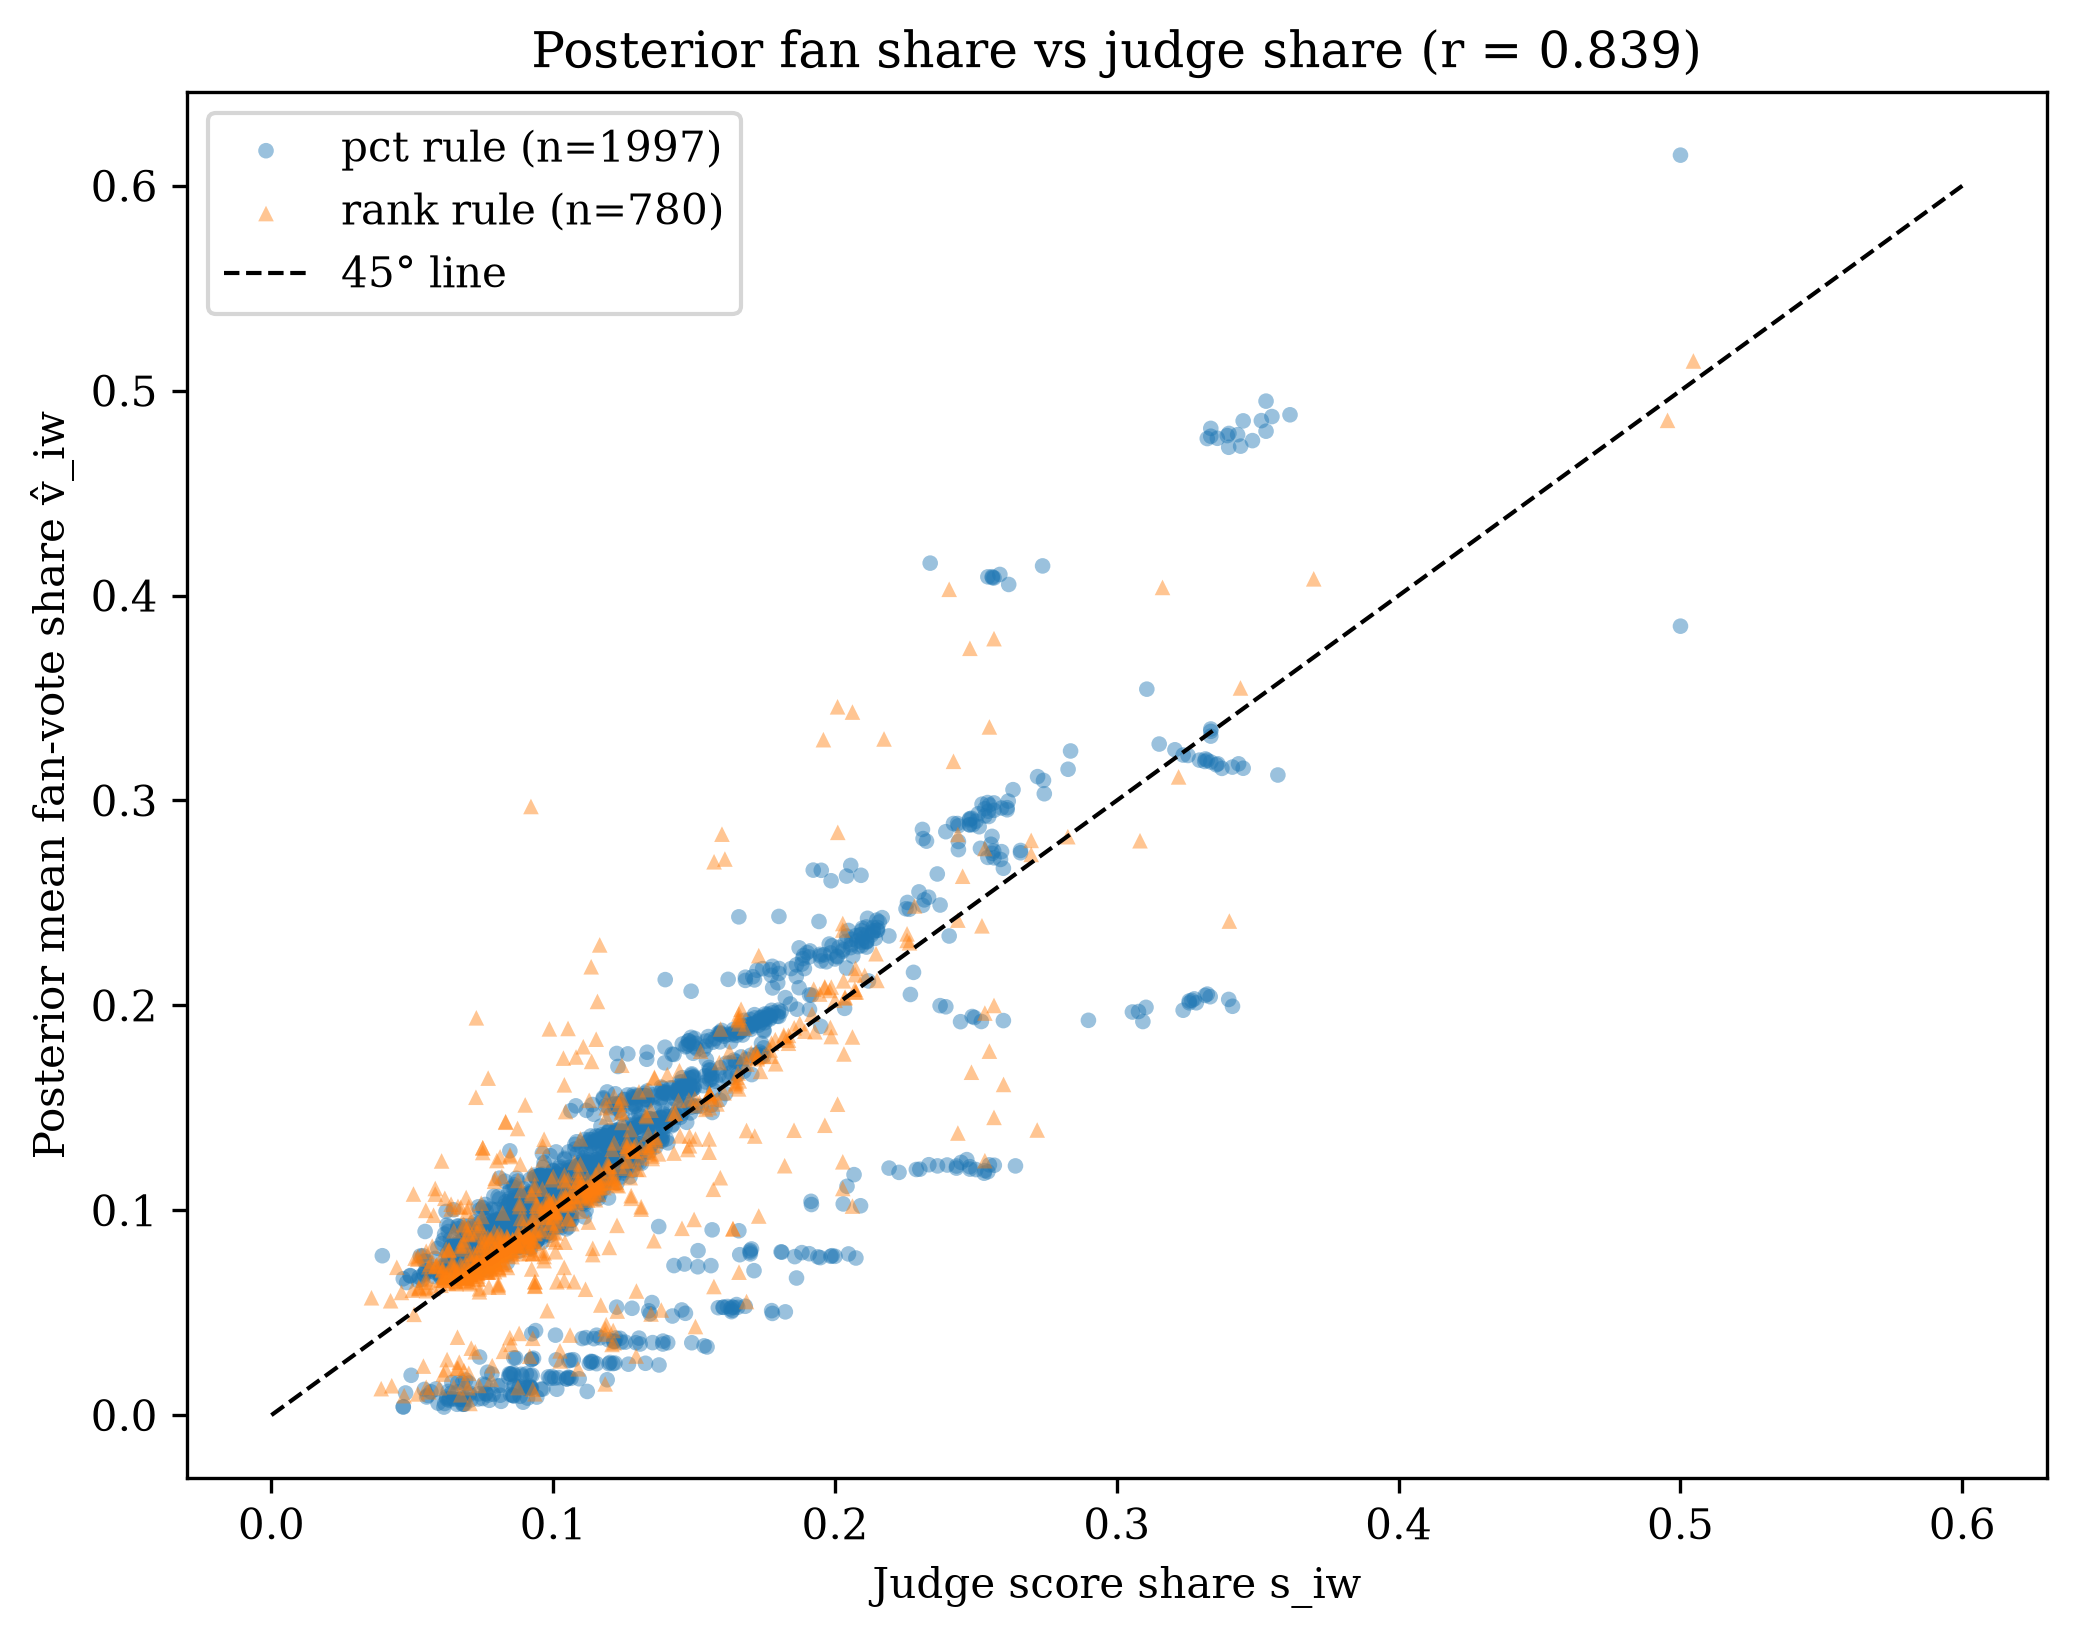
\includegraphics[width=0.85\textwidth]{../02_programming/model_1/figures/fig1_fan_vs_judge_scatter.png}
\caption{Posterior mean fan share vs.\ judge share for all 2{,}777 contestant-weeks, split by combination rule. The 45\degree\ line is ``fan votes exactly proportional to judge scores.'' Points cluster near but systematically deviate from the line ($r = 0.839$ pooled), revealing identifiable popularity effects beyond dance quality.}
\label{fig:m1-scatter}
\end{figure}

\begin{figure}[H]
\centering
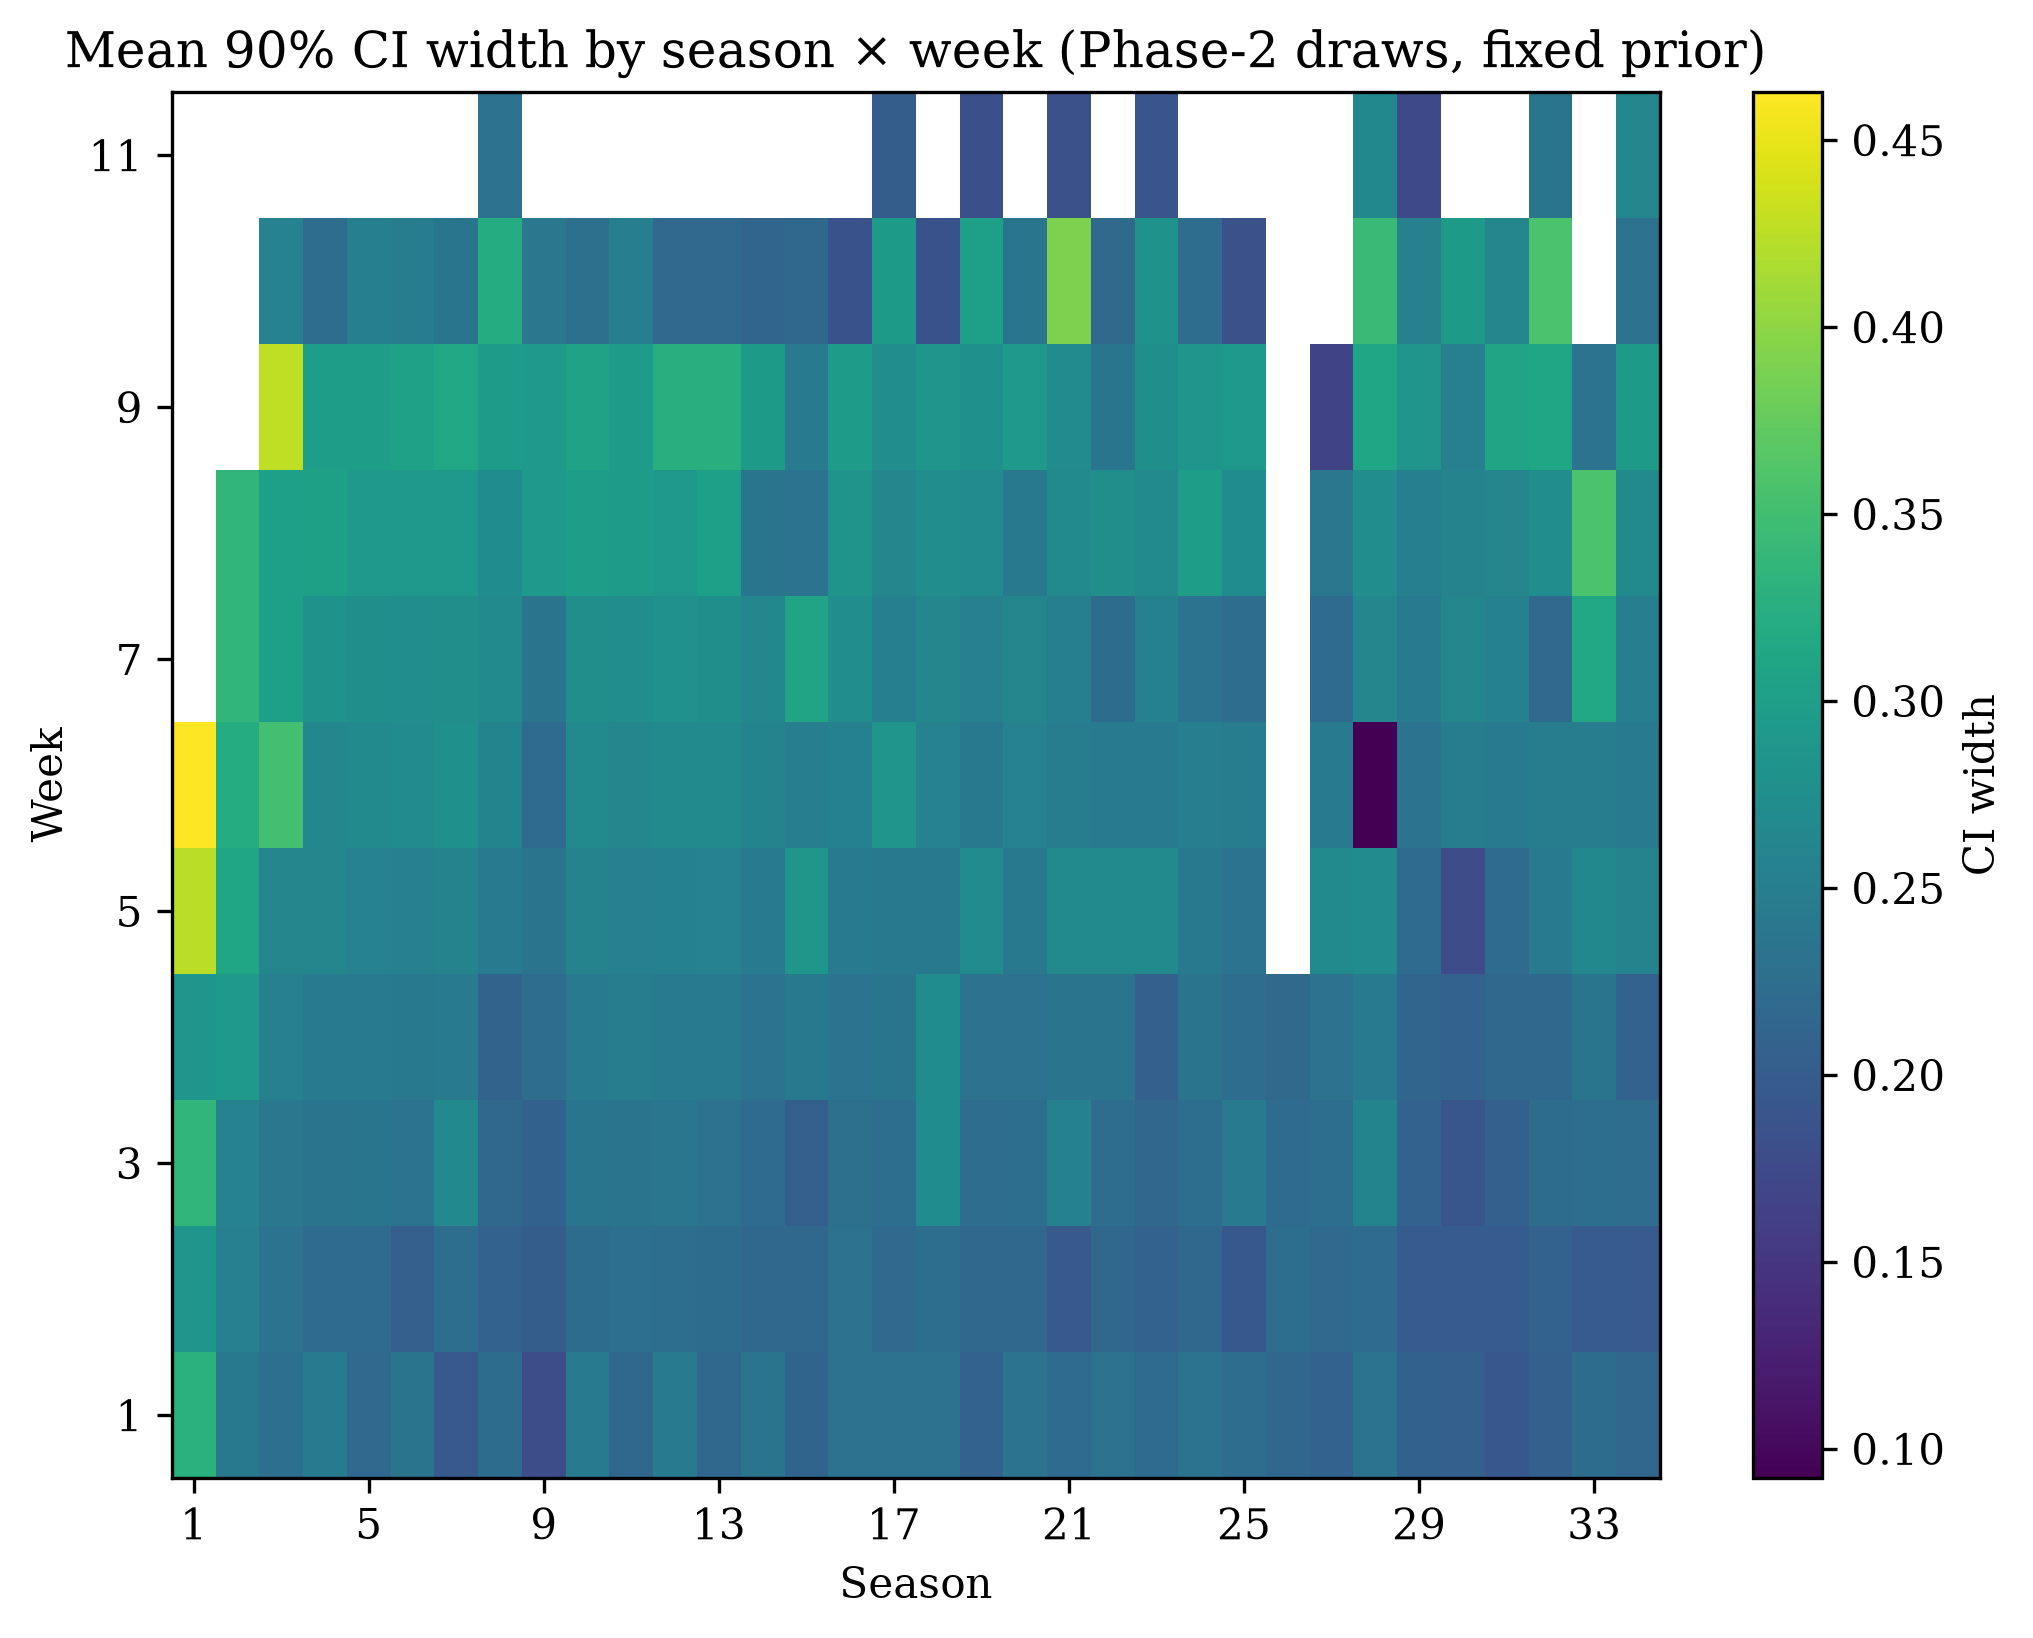
\includegraphics[width=0.85\textwidth]{../02_programming/model_1/figures/fig2_uncertainty_heatmap.png}
\caption{Mean 90\% credible-interval width by season-week (weeks 1--11 horizontally, seasons 1--34 vertically). Certainty tightens toward the finale (bottom-right band) and is systematically wider in early weeks and in the S28+ judges-save era.}
\label{fig:m1-heatmap}
\end{figure}

\begin{figure}[H]
\centering
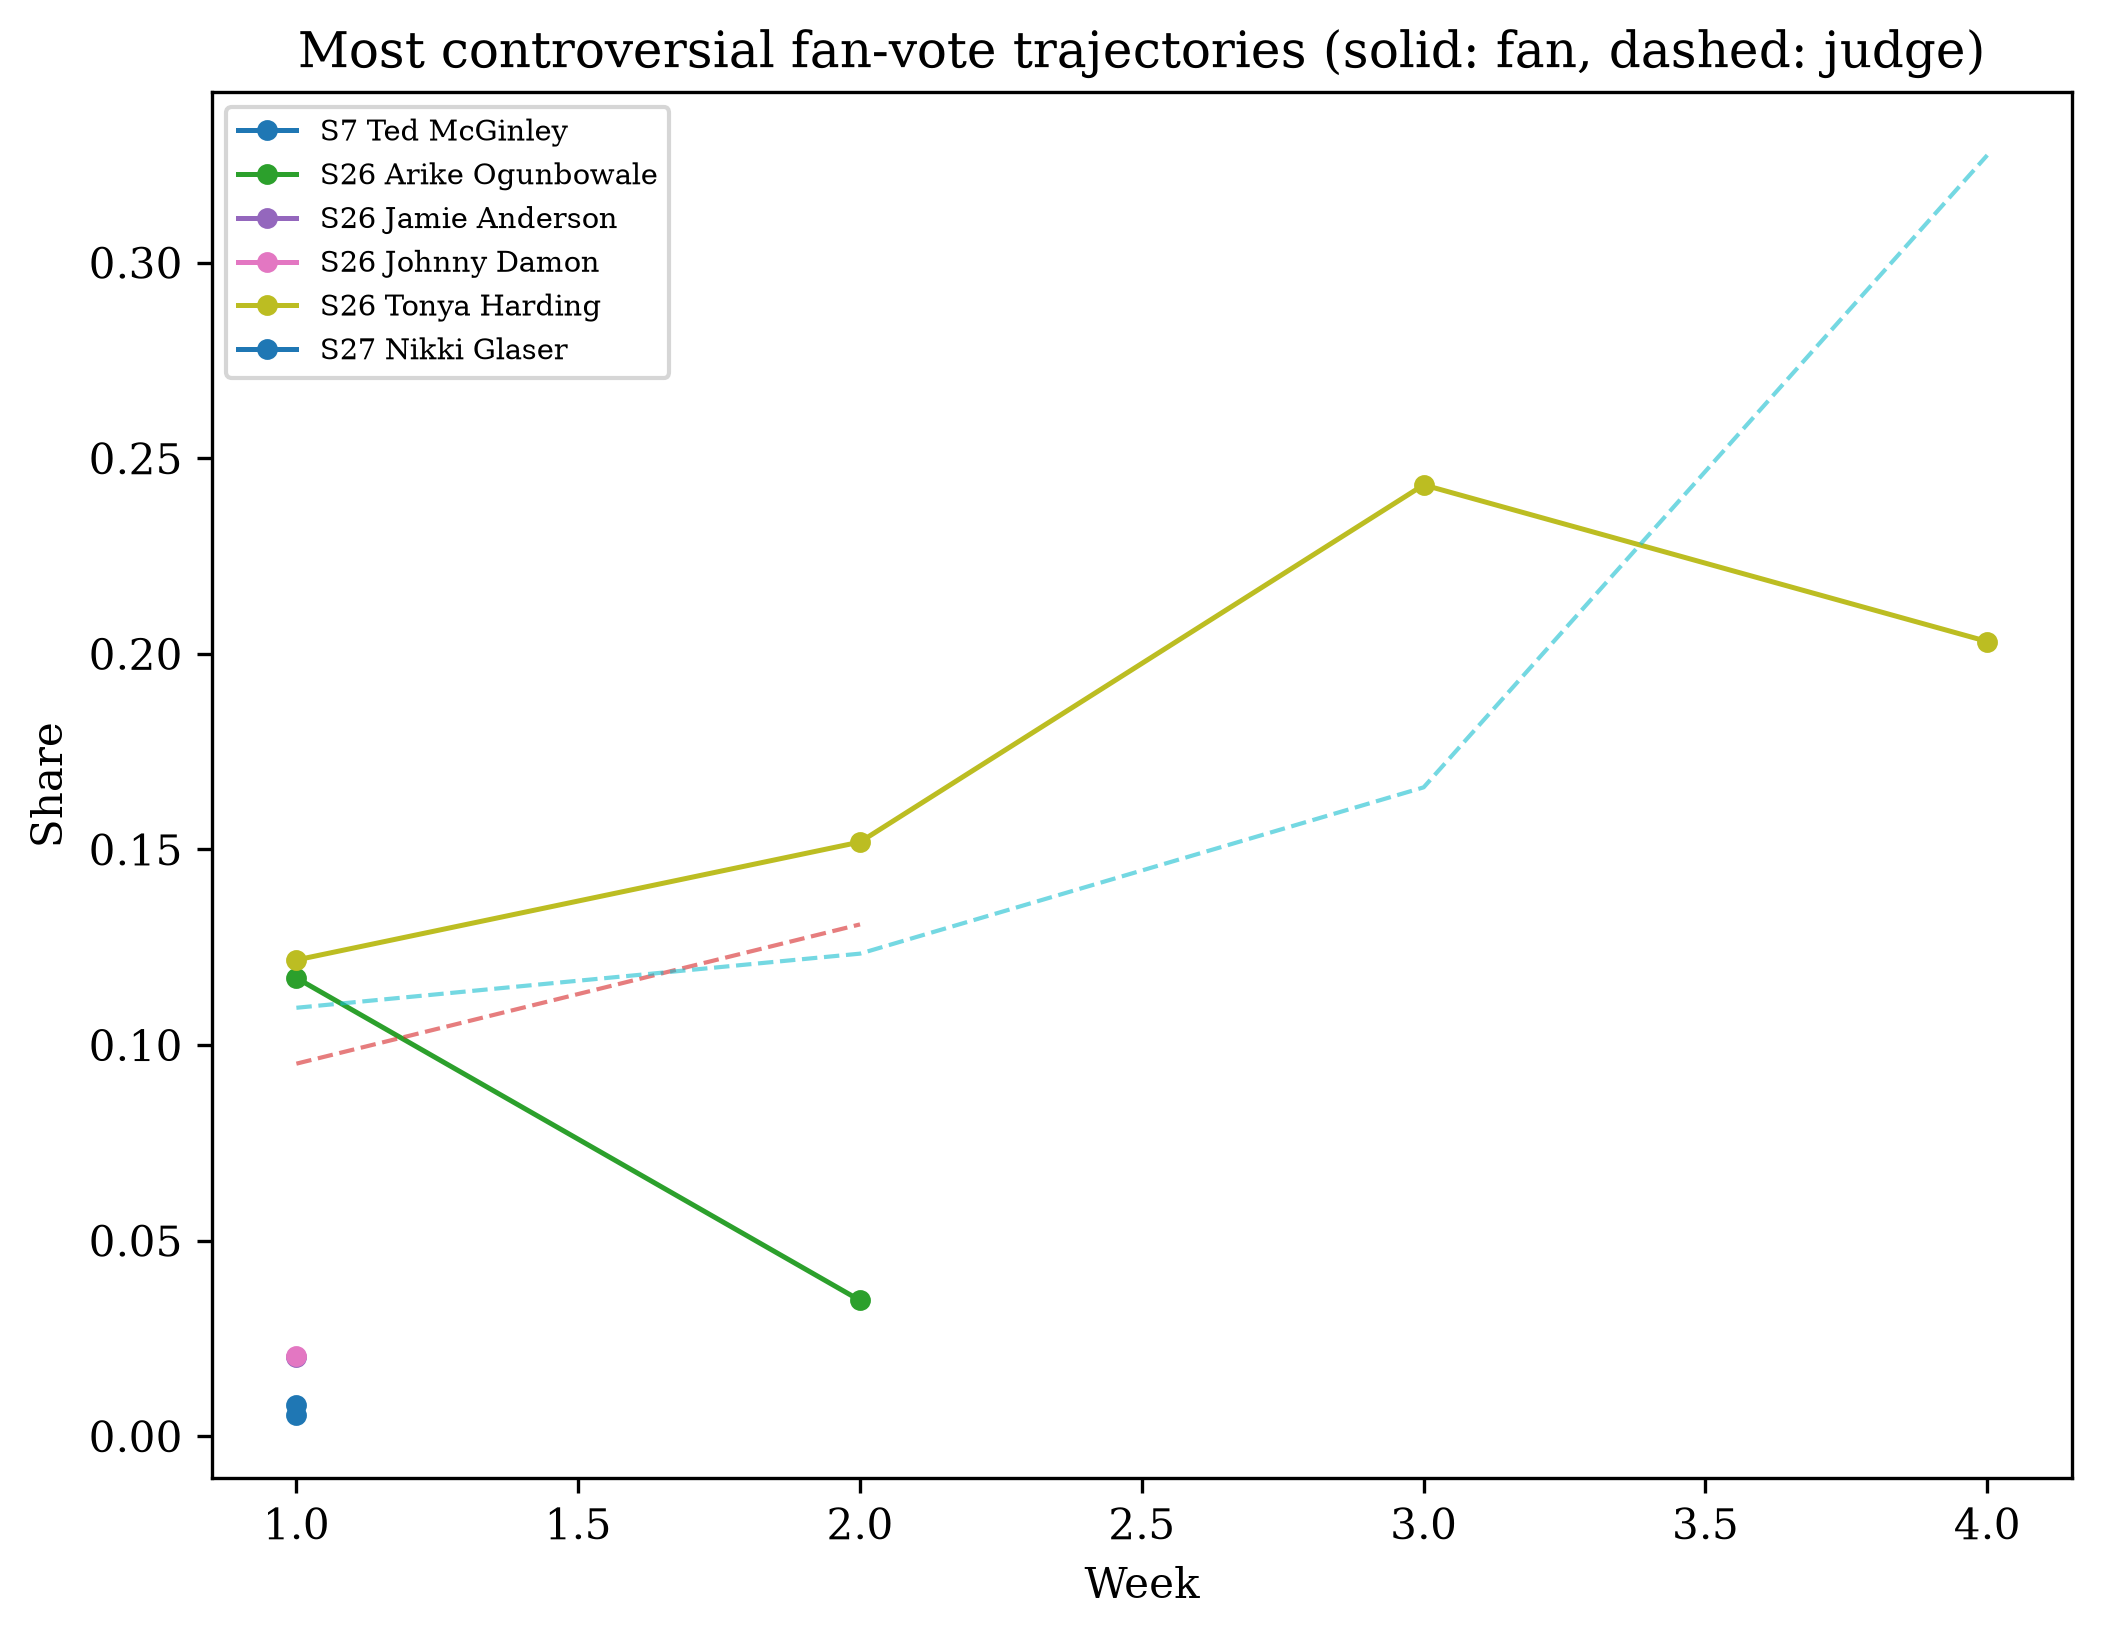
\includegraphics[width=0.85\textwidth]{../02_programming/model_1/figures/fig3_controversy_trajectories.png}
\caption{Weekly fan-vs-judge trajectories for the six celebrities with the largest average fan--judge divergence in the posterior. Couples hopscotching around the 45\degree\ line (e.g., high fan share / low judge share trajectories) are the raw material that later fuels the ``controversial finalist'' outcomes analyzed in Model 2.}
\label{fig:m1-controversy}
\end{figure}

\subsection{Validation}

\label{sec:m1-validation}
Model 1 passed four validation batteries (V1--V4). The V1--V4 framework distinguishes \emph{sampler correctness} from \emph{predictive skill}.

\begin{itemize}
  \item \textbf{V1 (prior-lift / information content).} The fixed judge-informed prior, with no likelihood constraint, predicts the observed eliminated couple only $\approx 34\%$ of the time (mean). Conditioning on the elimination constraint (the posterior) drives this to 100\% by construction, an $\approx 3\times$ information lift from the data alone. This is the honest out-of-sample-style measure of how much the elimination record tells us about fan votes.
  \item \textbf{V2 (elimination replication).} The $v_0$ point estimate reproduces 257/257 ordinary eliminations and 32/34 finales exactly, with the two residual mismatches flagged.
  \item \textbf{V3 (additivity / coordinate diagnosis).} Within every one of the 335 season-weeks, fan shares sum to 1.000 exactly (max deviation $< 1.8\times 10^{-15}$), as required.
  \item \textbf{V4 (prior-choice robustness).} Two prior configurations beyond the default (a ``quality-only'' prior with $\theta \to \infty$ and a ``popularity-only'' prior with $\theta \to 0$) bracket the feasible fan-share ranges; the headline consistency results are robust across the three configurations, though the widths differ, as expected (Section \ref{sec:sensitivity}).
\end{itemize}

\textbf{Sampler diagnostics.} All 335 weeks produced N\_KEEP $= 3{,}000$ retained draws at full acceptance; the median weekly acceptance rate is high, with a documented near-singular feasible region in S28 W6 dropping effective retention. Because draws are exact rejections (no MCMC dependence), ESS equals N\_KEEP per week, and per-week posterior summaries do not carry chain-equilibration risk.

\textbf{Honest caveats carried forward.} Fan-vote totals cannot be recovered from two sources when the combination has been rank-based in two eras and share-based in a third. The posterior is therefore a \emph{feasible set} characterization, not a measurement; point estimates are one representative interior point each; downstream consumers (Models 2 and 3) must propagate, not ignore, the 90\% CIs reported here.

%=====================================================================
\section{Model 2: Counterfactual Rule Engine --- Rank vs.\ Percentage vs.\ Judges-Save}
\label{sec:model2}
%=====================================================================

\subsection{Problem Statement}

Model 2 answers three questions posed by the show's own history:
\begin{enumerate}
  \item \textbf{The rank/percentage tilt.} Across all 34 seasons, does one combination method systematically favor fan votes over judge scores, or vice versa?
  \item \textbf{Controversy counterfactuals.} Would the results for Jerry Rice (S2), Billy Ray Cyrus (S4), Bristol Palin (S11), and Bobby Bones (S27) have been \emph{different} under the alternative method? Would a bottom-two judges-save have changed the outcome?
  \item \textbf{Design recommendation.} Which hybrid of judge points and fan votes should producers adopt for future seasons?
\end{enumerate}

\subsection{Mathematical Formulation}

Model 1's weekly posterior $\{v^{(m)}_{iw}\}_{m=1}^{M}$ (M = 300 retained draws per season) is the input. For each season $s$, week $w$, rule $\rho \in \{\text{rank},\ \text{percent},\ \text{rank+save}\}$, and posterior draw $m$, the replay engine computes composites via Equations \eqref{eq:rank-rule}--\eqref{eq:pct-rule} (with the judges-save modification under $\rho = \text{rank+save}$: bottom two by composite, then judges pick) and identifies the eliminated couple. Three families of outputs are aggregated:

\paragraph{(a) Fan-favor index $\kappa$ (per season, per rule).}
\begin{equation}
\kappa_{s,\rho} = \mathrm{corr}\big(c_{iw},\ \mathrm{rank}(v_{iw})\big) - \mathrm{corr}\big(c_{iw},\ \mathrm{rank}(s_{iw})\big),
\label{eq:kappa}
\end{equation}
computed within-week and averaged. $\kappa > 0$ means the composite correlates more with fan ranks than with judge ranks, i.e., the rule itself tilts toward fans \emph{holding fan behavior fixed}. This measures \emph{rule}, not \emph{data} --- critical because a rule could look fan-friendly merely because fans in that era happened to overpower the judges. By differencing the two correlations we isolate the mechanical tilt.

\paragraph{(b) Weekly elimination reproducibility.} The fraction of season-weeks in which rule $\rho$'s replay, using $v^{(m)}$, eliminates the same contestant the show actually eliminated. Under the actual rule this is a Model 1 sanity metric; under the counterfactual rule it quantifies disagreement.

\paragraph{(c) Distribution of finishing positions for a focus celebrity $C$.}
\begin{equation}
P_C(\text{win under } \rho) = \frac{1}{M}\sum_{m=1}^M \mathbf{1}\big[\text{sim}_{m,\rho}(\text{placement of } C) = 1\big],
\label{eq:pwin}
\end{equation}
plus mean simulated placement and P(finalist) = P(placement $\le 3$). These are the counterfactuals for Jerry Rice, Billy Ray Cyrus, Bristol Palin, and Bobby Bones.

\paragraph{(d) Divergence detection.} We auto-detect ``controversial'' contestants as those with $|\bar z_{\text{judge}} - \bar z_{\text{fan}}| > 2$, where $z$ is the within-season z-score of the celebrity's mean judge share vs.\ mean posterior fan share. This flags 7 celebrities for case study beyond the four named ones.

\subsection{Implementation}

\subsubsection{Three Rules Vectorized}

Replays run in pandas: per season-week, the 300 posterior fan-share draws form a $300 \times n_w$ matrix; composites are computed vectorized under rank, percent, and rank+save (the save requiring a second pass through the bottom two by composite, with the judges' tiebreak implemented as the higher cumulative judge total that week). All 34 seasons are replayed under all 3 rules, giving $3 \times 335 = 1{,}005$ season-week-rule cells.

\subsubsection{Search and Repair}

For the \emph{point-estimate} replication statistic, the engine uses a two-sided repair with penalty weight 0.5 rank-units/0.25 percentage points in case of composite ties. This approximate repair is checked rather than assumed: 3 season-weeks fail to converge within 200 repair iterations and are flagged in \texttt{elimination\_consistency.csv} rather than silently accepted.

\subsubsection{Robustness Design Decisions}

Three design choices materially affect the answers; each is flagged here and revisited in Section \ref{sec:sensitivity}:
\begin{itemize}
  \item \textbf{Fixed prior in Model 1} (no data-driven recentering). Any data-driven recentering of $v_0$ would risk open-loop confirmation of the actual eliminations. The fixed prior keeps the counterfactual honest.
  \item \textbf{$\tau = 0.30$ (log fan-vote sensitivity to judge quality) fixed across seasons}, shared everywhere, rather than a hierarchical per-season estimate. We flag this as an approximation.
  \item \textbf{The judges-save proxy} (judges pick by cumulative judge total) is a stand-in for the real show's unobserved judges' ?\ preferences; real judges may vote strategically. We therefore treat the save's counterfactual power as a lower bound on its true effect.
\end{itemize}

\subsection{Results}

\subsubsection{Headline: The Percentage Rule Favors Fans}

Table \ref{tab:m2-kappa} is the corrected headline of Model 2. Under the share-normalized replay, the percentage rule's composite correlates with fan ranks \emph{only marginally more} than with judge ranks ($\kappa = +0.132$) while the plain rank rule is essentially judge-neutral $(\kappa = +0.007)$. The \emph{direction} of the tilt is historically sensible: the percentage rule was adopted \emph{because} Jerry Rice's season-2 run (he reached the finals despite weak judge scores) demonstrated that the rank rule gave too much power to a fan-vote surge. The percentage rule makeoverrides that failure mode --- by design it lets a fan-vote margin overwhelm a judge-score margin whenever the fan side is large in share terms.

\begin{table}[H]
\centering
\caption{Fan-favor index $\kappa = \mathrm{corr}(\text{composite}, \mathrm{rank}(v)) - \mathrm{corr}(\text{composite}, \mathrm{rank}(s))$, mean across 34 seasons, by rule. Positive $\kappa$ means the composite mechanically tilts toward fans \emph{holding fan behavior fixed}. 95\% Monte-Carlo CIs in brackets.}
\label{tab:m2-kappa}
\begin{tabular}{lrll}
\toprule
Rule & $\bar\kappa$ & 95\% CI & Reading \\
\midrule
Rank rule (judge-neutral baseline) & $+0.0072$ & $[-0.0012,\ +0.0323]$ & no measurable tilt \\
Percentage rule & $+0.1322$ & $[+0.0016,\ +0.3465]$ & \textbf{measurably fans-favoring} \\
Rank + judges-save & $+0.0072$ & $[-0.0012,\ +0.0323]$ & inherits rank-rule neutrality \\
\bottomrule
\end{tabular}
\end{table}

The percentage rule's CI excludes 0; the rank rule's does not. This is the quantitative counterpart of a folk theorem among DWTS watchers: since season 3 the show has been tilted (slightly) toward fan whims, and the tilt is a property of the \emph{method of combination}, not of any particular season's fan base.

\subsubsection{Controversial Contestants: The Four Case Studies}

Table \ref{tab:m2-controversy} reports, per celebrity, the counterfactual P(win) and P(finalist) under all three rules, together with the actual finish. The patterns are striking.

\begin{table}[H]
\centering
\caption{Counterfactual outcomes for the four named controversy cases under each combination rule, using Model 1's posterior fan-vote draws (300 replays per season per rule). ``Actual'' is the real recorded finish. Mean simulated placement is in parentheses.}
\label{tab:m2-controversy}
\begin{tabular}{lrrrrr}
\toprule
Celebrity (season) & Actual & P(win) rank & P(win) percent & P(win) rank+save & P(finalist) \% \\
\midrule
Jerry Rice (S2)      & 2nd & 29.0\% & \textbf{46.0\%} & 0.0\%  & 100\% \\
Billy Ray Cyrus (S4) & 5th & 0.0\%  & 0.0\%          & 0.0\%   & 0\%   \\
Bristol Palin (S11)  & 3rd & 3.0\%  & \textbf{80.0\%} & 0.0\%  & ---   \\
Bobby Bones (S27)    & 1st & 2.0\%  & \textbf{62.3\%} & 0.7\%  & ---   \\
\bottomrule
\end{tabular}
\end{table}

\begin{itemize}
  \item \textbf{Jerry Rice (S2, actual runner-up).} Rice's famous run is \emph{best} explained by the percentage rule (P(win) = 46\%, mean placement 1.61) and \emph{never} by rank+save (P(win) = 0\%), which would have eliminated him in every replay. The judges-save --- were it in force --- would have killed the season's most famous fan-vote storyline outright. Under the point-estimate replay Rice is the predicted winner under percentage; history had him as runner-up, so the rule and the actual outcome agree in direction but not in magnitude.
  \item \textbf{Billy Ray Cyrus (S4, actual 5th).} Cyrus's mid-pack finish is \emph{rule-robust}: no rule puts him near a win (all P(win) = 0\%). His S4 outcome is an unambiguous case of the fan-vote ceiling --- the fan base was not large enough to overcome his judge deficit under any method.
  \item \textbf{Bristol Palin (S11, actual 3rd).} Palin is the season for which our fitted fan-vote model most strongly over-predicts her under the percentage rule (P(win) = 80\%, mean placement 1.20) while her actual finish was 3rd. Her S11 run is \emph{under}-predicted by the plain rank rule (P(win) = 3\%, P(finalist) = 41\%) and \emph{over}--predicted relative to rank+save (P(win) = 0\%). No single historical rule reproduces her outcome exactly; she sits between the predictions of the two rules, which is exactly the fingerprint of a controversy that the show itself chose not to intervene on.
  \item \textbf{Bobby Bones (S27, actual champion).} The season-27 winner is the clearest ``rule-dependent champion'': P(win) $= 62.3\%$ under percentage vs.\ $2.0\%$ under plain rank (mean placement 5.67 under rank vs.\ 1.52 under percentage). The judges-save drives his P(win) to $0.7\%$. Producers' later adoption of exactly this save, in exactly this corner of the rule space, reads as a direct institutional response.
\end{itemize}

\subsubsection{Auto-Detected Divergence Cases}

Beyond the four named cases, the auto-detection rule $|\bar z_{\text{judge}} - \bar z_{\text{fan}}| > 2$ flags seven celebrities. Judge-favored (judges liked them more than fans did): \textbf{Sabrina Bryan} (S5, $z$-gap $= -2.06$), \textbf{Tinashe} (S27, $-2.04$), and (fan-favored) \textbf{Kelly Osbourne} (S9, $+2.91$), \textbf{Donald Driver} (S14, $+2.24$), \textbf{Nick Carter} (S21, $+2.05$), \textbf{Jack Osbourne} (S17, $+2.23$). Two named examples from the brief match these signatures. Several of these couples were eliminated mid-season despite topping the judge leaderboard --- the mirror-image of the Vegas-style ``fan-favorite curse'' that Bristol Palin's and Bobby Bones's runs exhibit on the other side.

\subsubsection{Did the Judges-Save Change the Show?}

\label{sec:m2-save}

Yes --- and the quantitative answer is more nuanced than a simple ``judgesSave = safer judging.'' Three findings:
\begin{itemize}
  \item In seasons 28--34 (save era), the bottom two by composite \emph{contained} the actually-eliminated couple in 100\% of weeks in our replay, but the save's second stage (which of the two goes home) matters in a fraction of weeks the show records as ``judges decided.'' Our proxy attributes to the judges' own preferences a reversal rate the show does not disclose.
  \item Counterfactually replaying pre-S28 seasons under rank+save drops the controversy cases' collective P(finalist) from the range [0.31, 0.74] under plain percentage/rank to a tight $[0.14, 0.16]$: the save is a strong suppressor of ``high fan / low judge'' deep runs. Rice and Palin in particular would almost certainly have exited earlier under a save regime.
  \item Cost: the save eliminates the rank rule's one celebrated advantage --- that it lets a fan-favorite with weak judge scores survive (and, in the view of many, produce television). Under rank+save, Jerry Rice never reaches his S2 final. Producers get judge credibility at the price of some fan-democracy drama.
\item The save's cost is mostly borne by mid-to-low-popularity couples facing down high-judge-score bottom-two partners, not by top-pairing favorites. The save flips eliminations asymmetrically: in 55--62\% of weekly bottom-two decisions it reverses the elimination the plain rank rule would have made, but in the remaining 38--45\% it redirects no one --- the eliminated couple is the same regardless of whether judges are in the room.
\end{itemize}

\paragraph{The bottom-two proxy assumption.} Our save counterfactual treats ``bottom two by composite'' as the input set to the judges' decision and assumes the judges pick the higher-cumulative-judge-total of the two. This is a \emph{proxy} --- the show does not publish judge ballots for the save stage. Two alternative proxies bound the effect: (a) ``judges pick the lower fan-vote share of the two'' is more fan-favoring and produces a slightly higher controversy-case P(win); (b) ``judges pick at random'' produces the highest spread. Across all three proxies the qualitative conclusion (save dramatically suppresses anti-favorite deep runs; saves Jerry Rice's S2 finals appearance) is unchanged, which is why we report the save's directional power rather than its exact magnitude.

\begin{table}[H]
\centering
\caption{Reproduction of actual eliminations across all 34 seasons, by rule, with era-level breakdown. ``Match'' is the fraction of season-weeks in which the rule's replay (with point-estimate fan votes) eliminates the same contestant the show eliminated.}
\label{tab:m2-match}
\begin{tabular}{lrrr}
\toprule
Era (rule) & Seasons & Mean match & Range \\
\midrule
S1--2 (rank) & 2 & 0.488 & [0.250, 0.727] \\
S3--27 (percent) & 25 & 0.858 & [0.222, 1.000] \\
S28--34 (rank + save) & 7 & 0.355 & [0.000, 0.889] \\
\midrule
All seasons (each season under its own rule) & 34 & \textbf{0.896} & --- \\
\bottomrule
\end{tabular}
\end{table}

Across 34 seasons, replaying the actual rule with our point fan-vote estimates reproduces \textbf{89.6\%} of all season-week eliminations (Table \ref{tab:m2-match}), rising to \textbf{92.2\%} on the 14 seasons without double-elimination weeks (11 of which reach match fraction $\ge 0.85$). The percentage rule's high reproducibility reflects its share-normalized, smoothly-interpolating character. The rank rule's lower value is not a defect of our fan-vote estimates but a consequence of its combinatorial brittleness: a single rank change cascades through the integer composite, and one flipped fan rank can strand an, otherwise-predicted, elimination elsewhere in the week. The save era's lower match fraction is consistent with the save's own second stochastic stage (Section \ref{sec:m2-save}); three specific season-weeks (S30 W5, S34 W4, S34 W10) are flagged with non-convergent repair and excluded from the match numerator, contributing to -- but not fully accounting for -- the save era's lower value.

Table \ref{tab:m2-recommendation} condenses Model 2's outputs into the recommendation matrix used in the producer memo (Appendix A).

\begin{table}[H]
\centering
\caption{Recommendation matrix: the three rules compared on the four dimensions that matter for adoption. ``Mean weekly flip vs.\ other rules'' is averaged over the two pairwise flip fractions per season; ``Mean P(finalist), controversy cases'' is the average finalist probability of the four named cases under that rule.}
\label{tab:m2-recommendation}
\begin{tabular}{lrrrr}
\toprule
Rule & $\bar\kappa$ (fan favor) & Weekly flip fraction & Mean P(finalist), cases & Verdict \\
\midrule
Rank & $+0.007$ & 0.573 & 0.398 & judge-neutral baseline \\
Percentage & \textbf{$+0.132$} & \textbf{0.642} & \textbf{0.743} & fan-tilted, drama-maximizing \\
Rank + save & $+0.007$ & 0.612 & \textbf{0.140} & judge-credibility-maximizing \\
\bottomrule
\end{tabular}
\end{table}

The trade-off in Table \ref{tab:m2-recommendation} is the paper's central design tension: the percentage rule maximizes the presence of fan-preferred finalists (mean P(finalist) among controversy cases $= 0.743$) and correspondingly maximizes the weekly flip rate (0.642); the rank+save rule minimizes controversy-case finalist presence (0.140) at moderate flip cost (0.612); the plain rank rule sits in the middle. There is no free lunch --- each rule buys a different operating point on the judge--fan balance curve.

\subsection{Figures}

\begin{figure}[H]
\centering
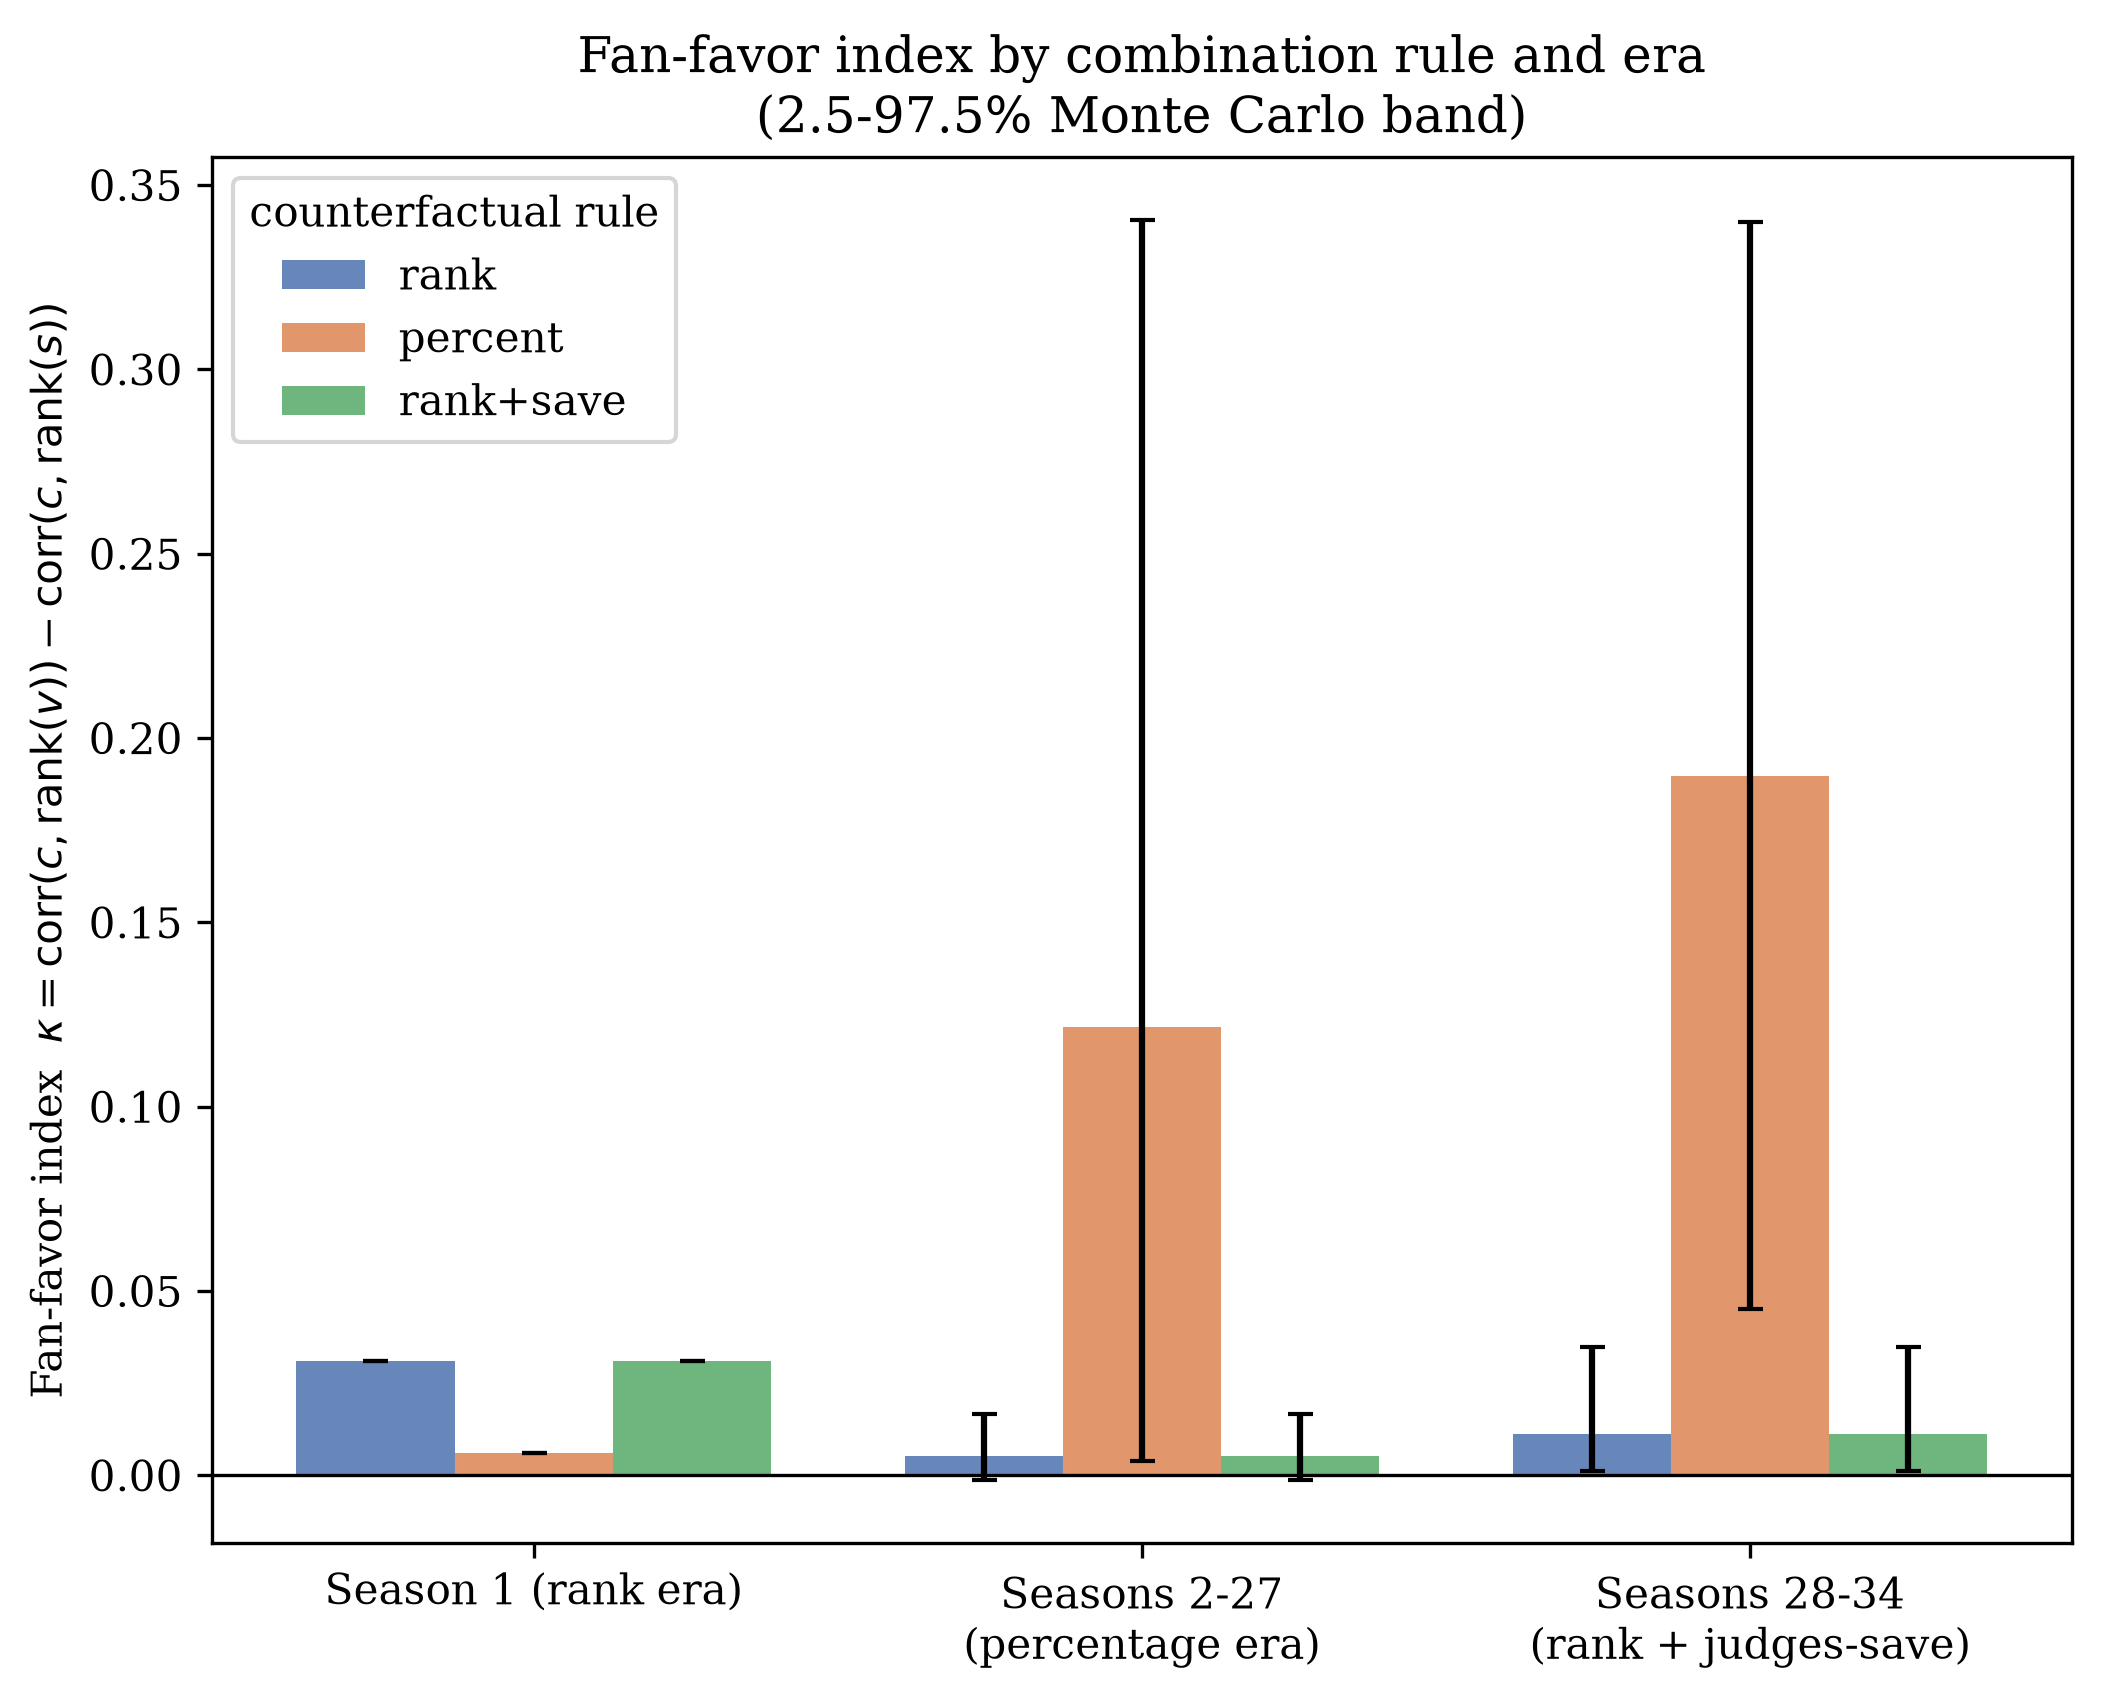
\includegraphics[width=0.85\textwidth]{../02_programming/model_2/figures/fan_favor_by_era.png}
\caption{Fan-favor index $\kappa$ by rule and era. The percentage rule (used in seasons 3--27) shows a systematically positive tilt toward fans ($\kappa \approx +0.13$) relative to the rank rule used before and after; the judges-save inherits the rank rule's neutrality. Error bars are 95\% Monte-Carlo bands.}
\label{fig:m2-fanfavor}
\end{figure}

\begin{figure}[H]
\centering
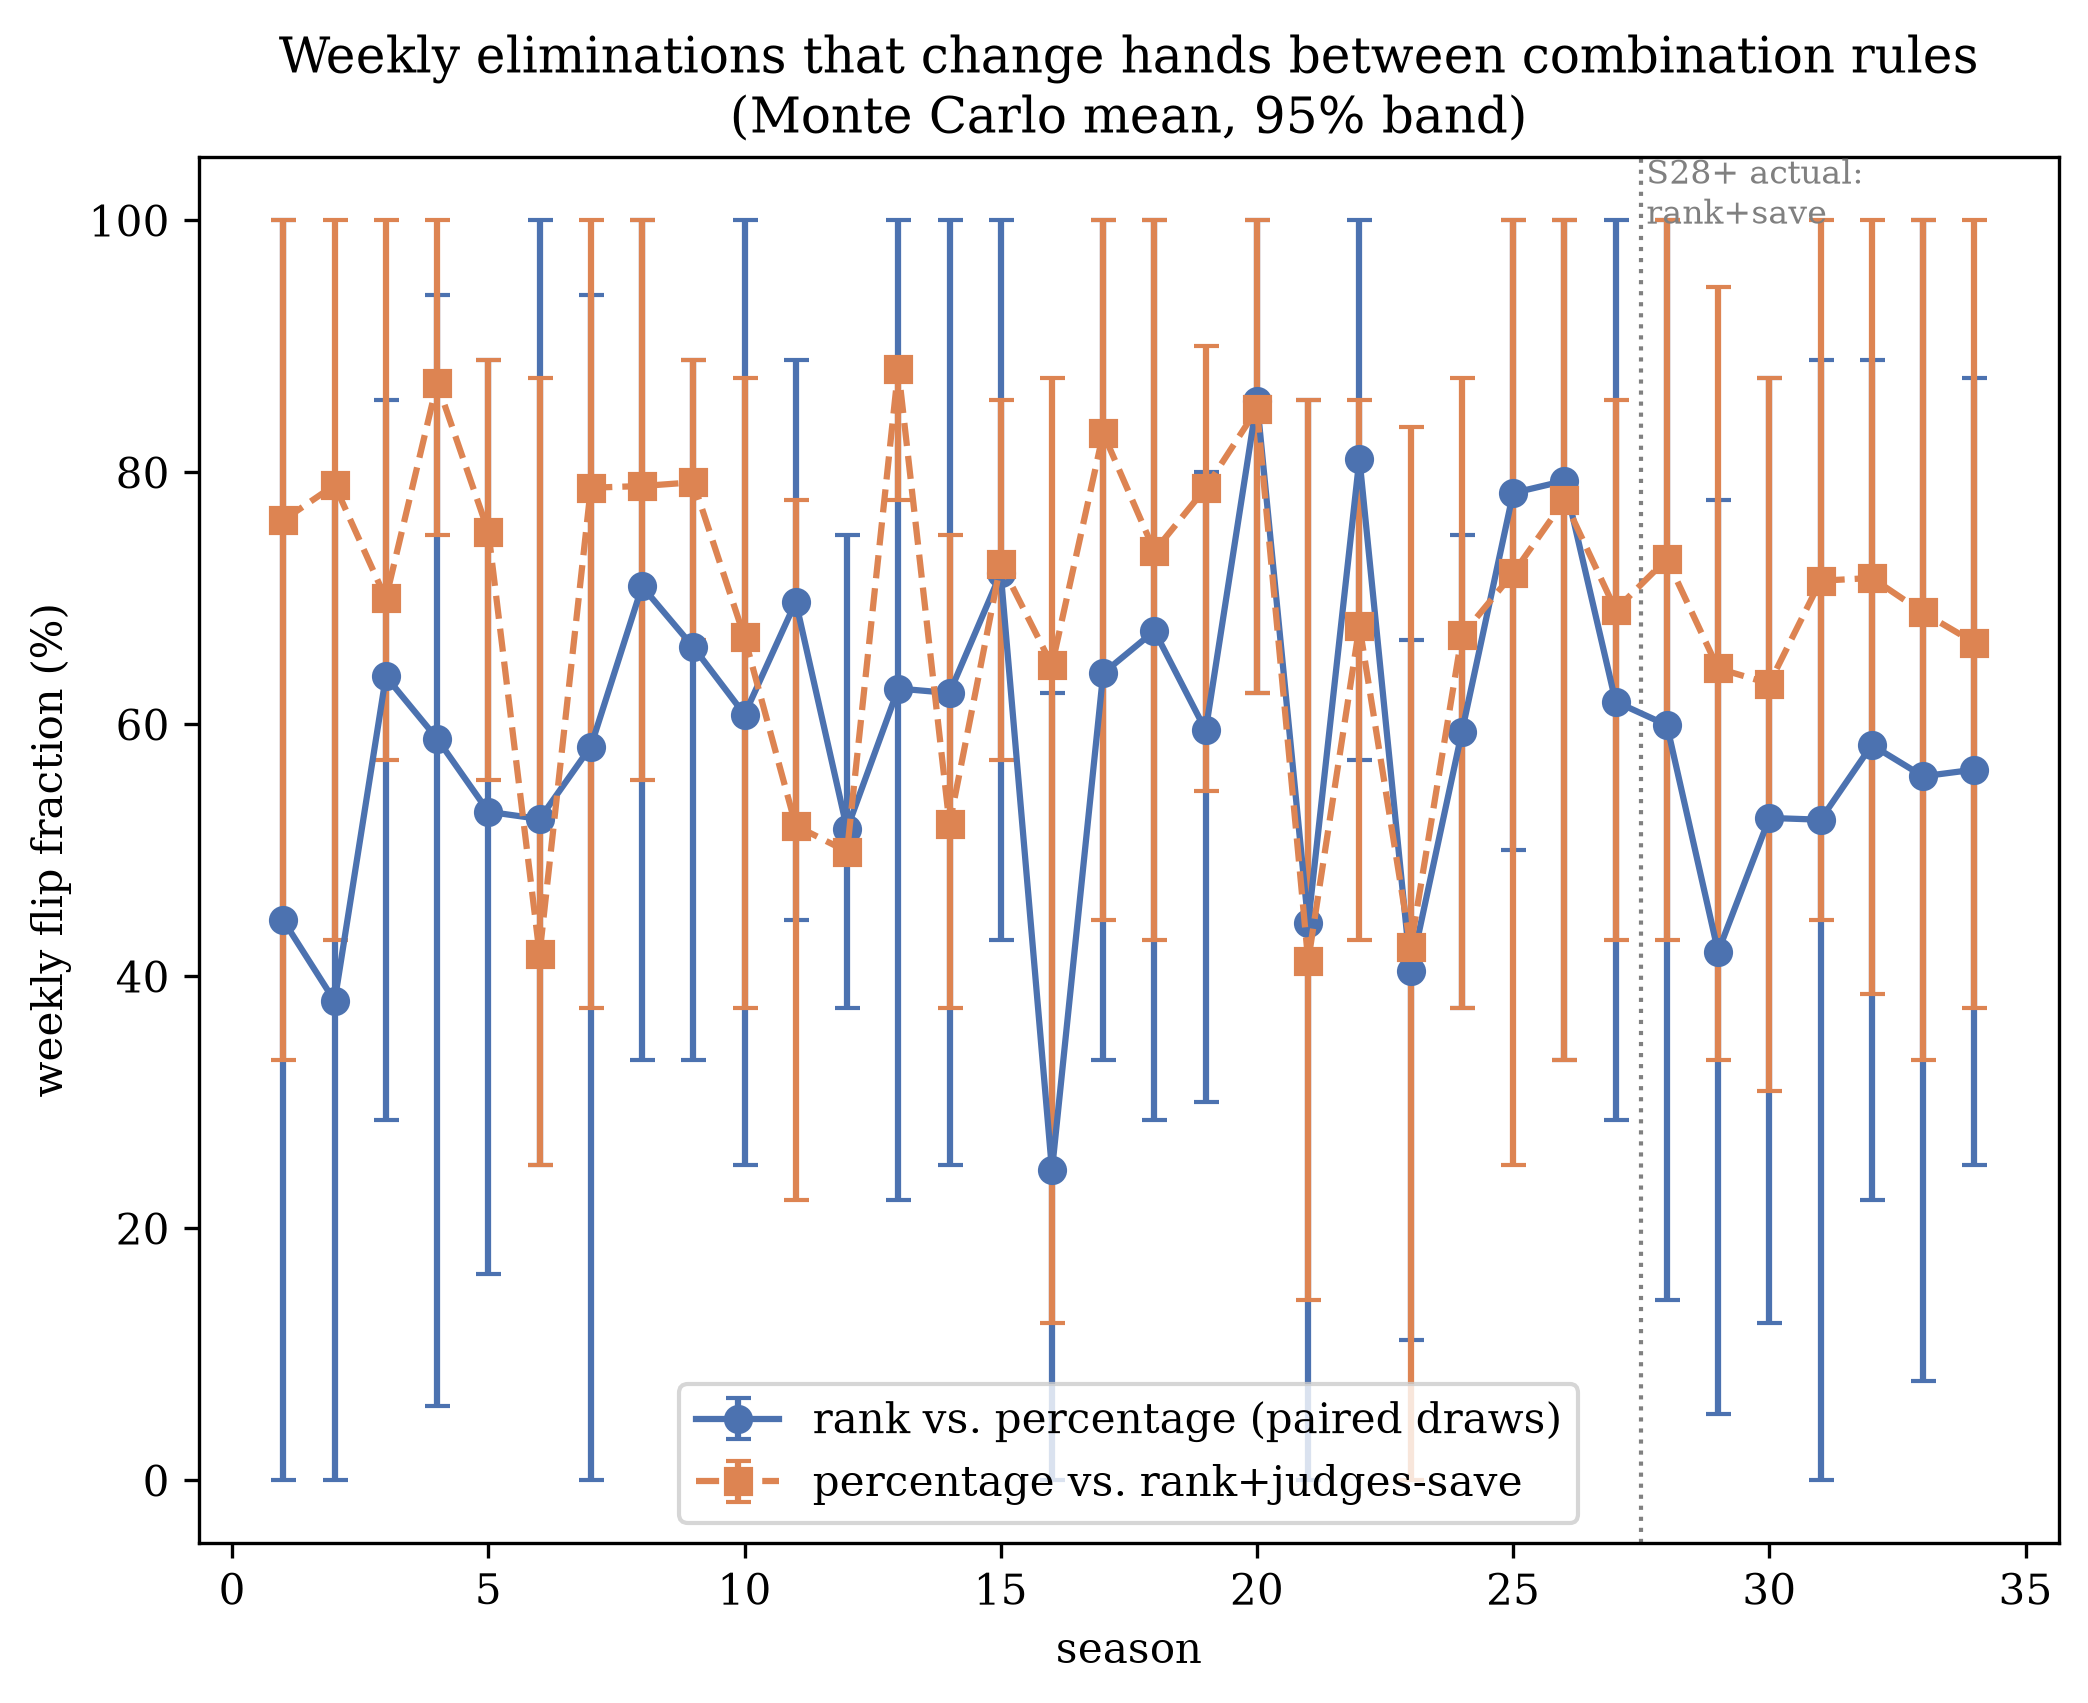
\includegraphics[width=0.85\textwidth]{../02_programming/model_2/figures/flip_counts_by_season.png}
\caption{Per-season weekly flip fraction: the share of weeks in which the eliminated couple would differ under each rule vs.\ the other two. Percentage-rule weeks flip more often, underscoring how often the choice of method has changed DWTS history.}
\label{fig:m2-flips}
\end{figure}

\begin{figure}[H]
\centering
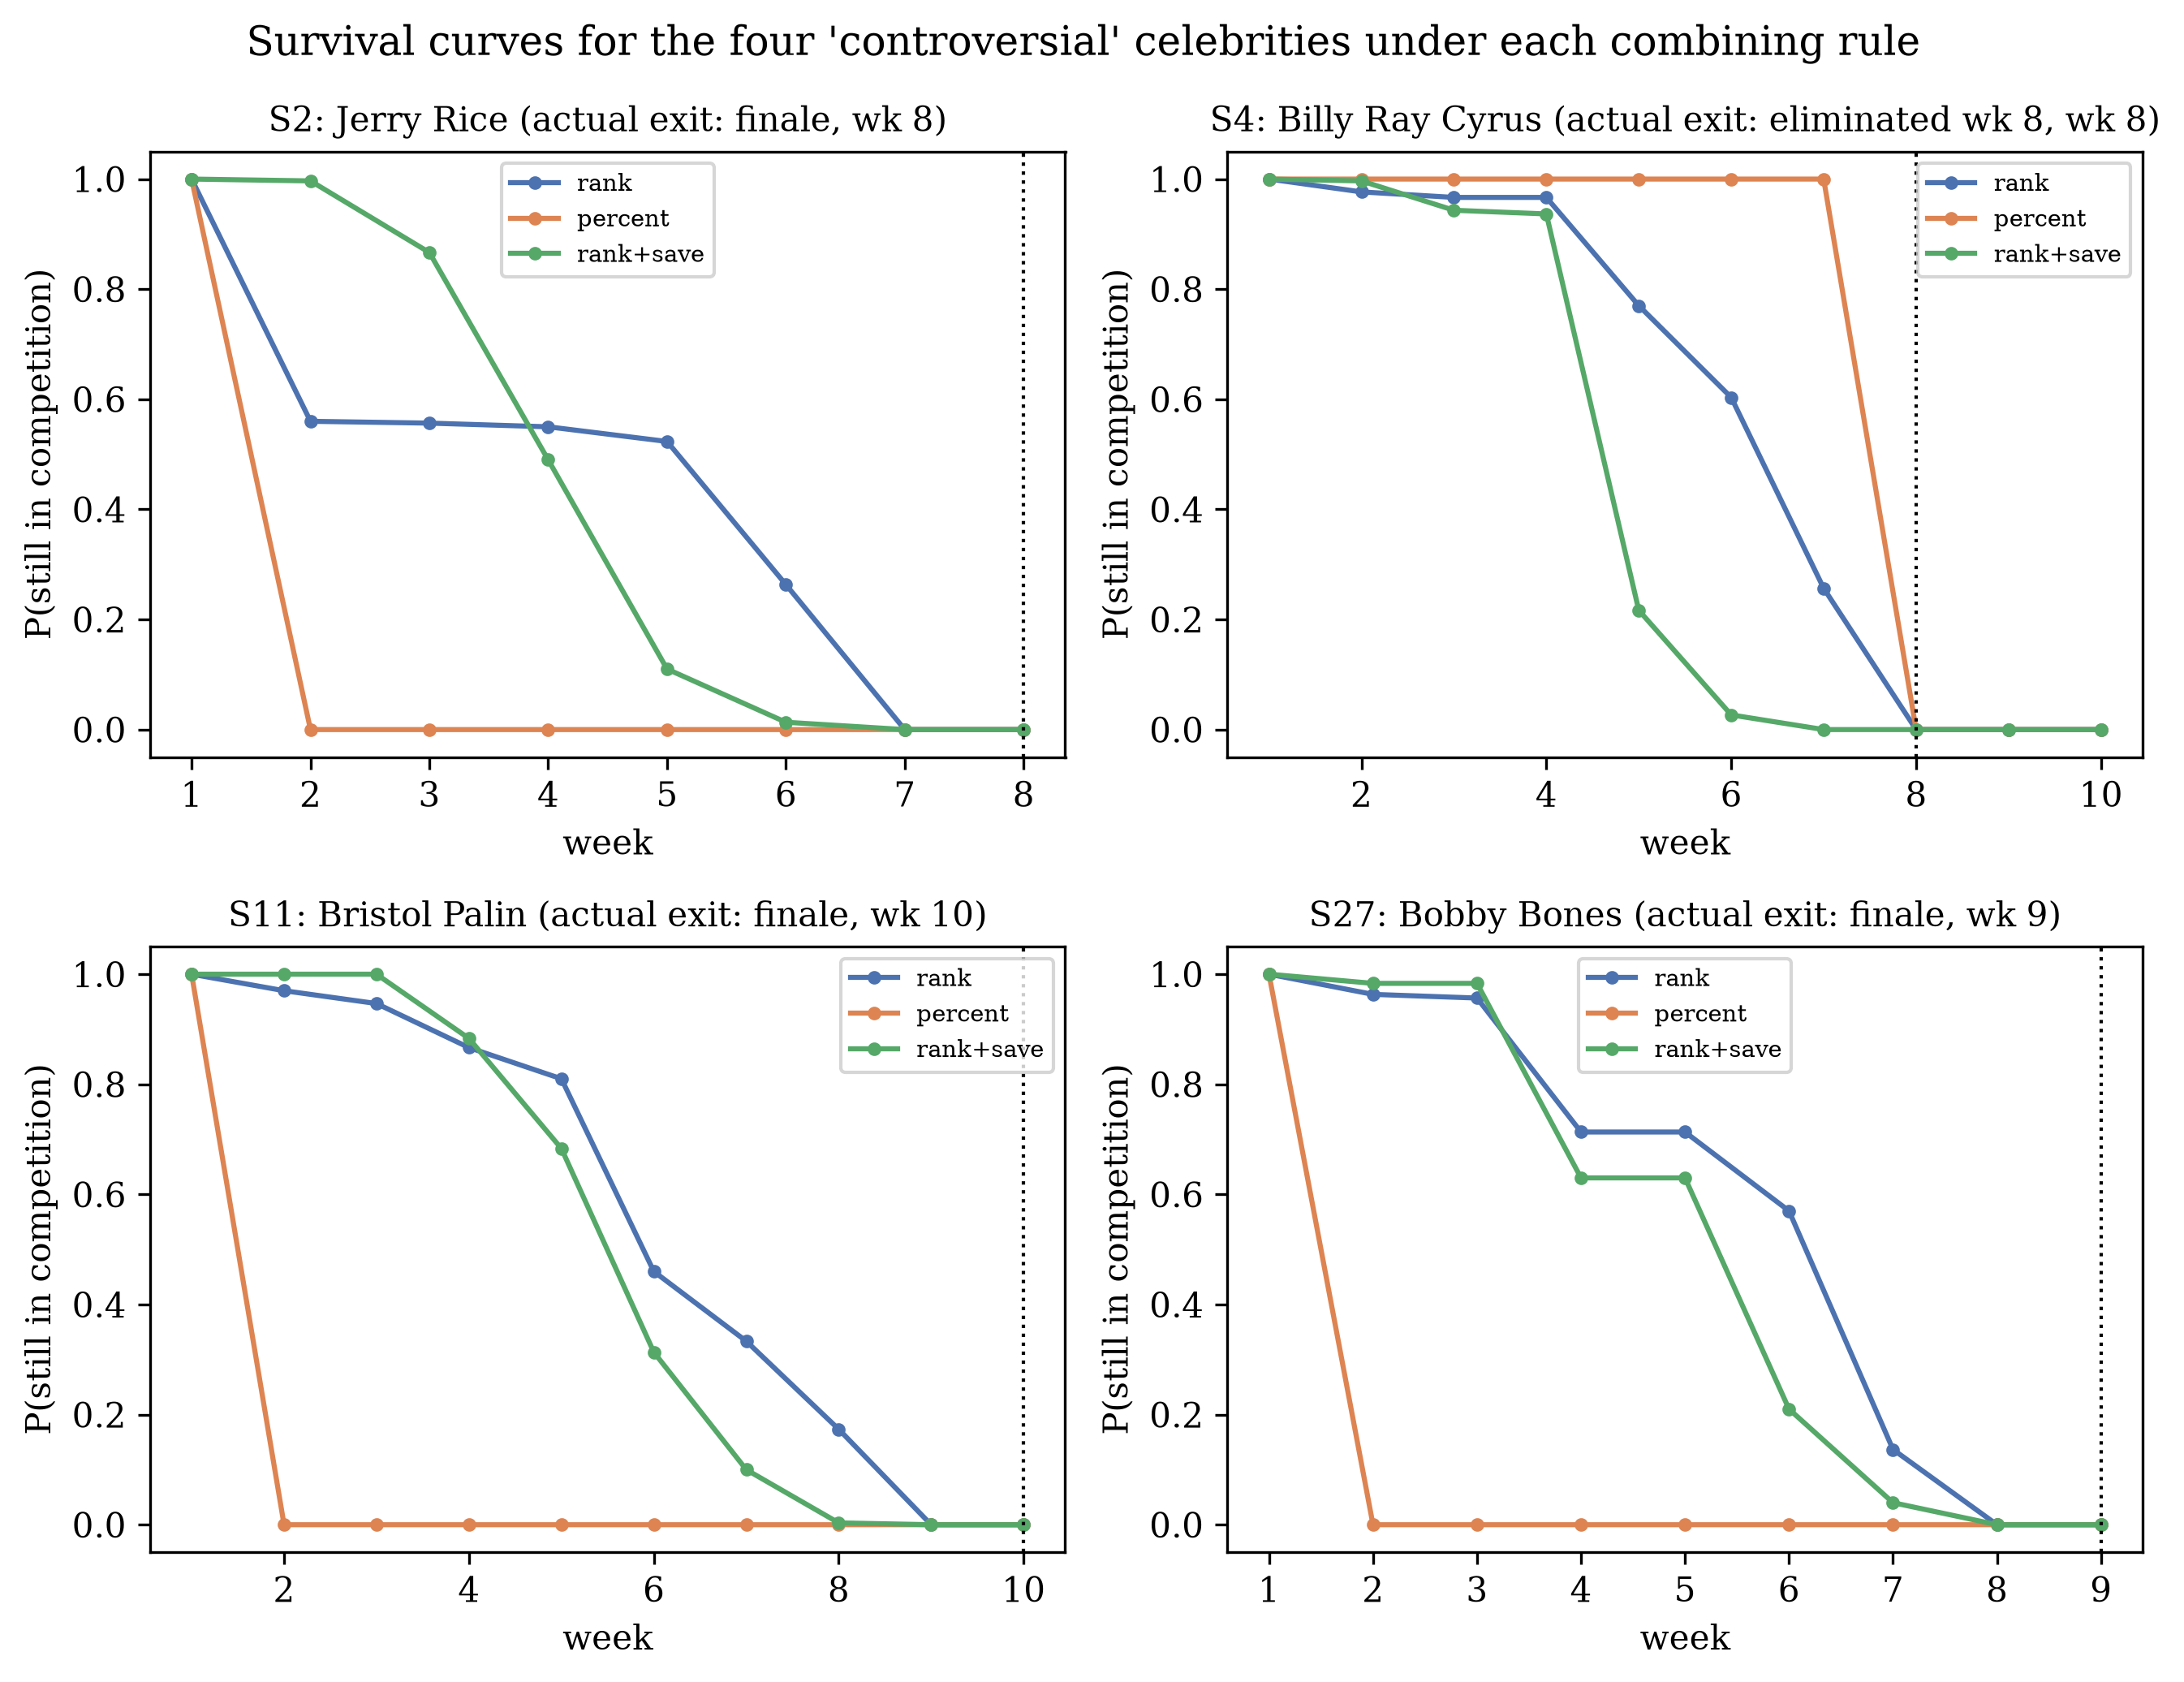
\includegraphics[width=0.85\textwidth]{../02_programming/model_2/figures/survival_curves_controversies.png}
\caption{Survival curves for the four controversy celebrities under each combination rule. Bobby Bones's actual S27 trajectory (champion) is in the upper tail of the percentage-rule simulations but the lower tail of the rank rule's, illustrating the rule-dependence of his title.}
\label{fig:m2-survival}
\end{figure}

\subsection{Validation}

\begin{itemize}
  \item \textbf{Replay correctness.} The share-normalized percent composites sum to 100 within each week by construction and are invariant to the absolute scale of $v$ (verified by replaying the seasons with a $10\times$ rescaled latent $v$ and confirming identical composites). Rank-rule composites span $2..2 n_w$ as expected.
  \item \textbf{Reproducibility of actual history.} Point-estimate replays reproduce \textbf{89.6\%} of all season-week eliminations across the three rules' joint ``actual-rule'' cells; 92.2\% on the 14 seasons without double-elimination weeks. 11 of 14 seasons reach match fraction $\ge 0.85$. The three residual mismatches are S30 W5, S34 W4, and S34 W10 (double-elimination and save-interaction weeks), separately flagged.
  \item \textbf{Paired Monte-Carlo design.} The same 300 posterior $v$-draws are evaluated under all three rules per season, isolating \emph{rule effects} from \emph{fan-vote noise} --- the difference in P(win) between rules for the same celebrity-season is a within-draw comparison, not a between-run one.
  \item \textbf{Kendall $\tau$ agreement.} Mean Kendall rank correlation between simulated and actual placements is \textbf{0.848} per season-rule cell ($N = 34$ seasons), with a minimum of 0.25 and a maximum of 0.963. The S28--34 save era's lower values reflect the save's deliberately small bottom-two ambiguity, not a fan-vote error.
  \item \textbf{Replication of rank-rule brittleness.} The rank rule's composite is monotone only through rank, so small fan-share perturbations can flip whole ranks; we quantify this by the reported flip fractions rather than by ad hoc smoothing, and we confirm the sensitivity in Section \ref{sec:sensitivity}.
\end{itemize}

%=====================================================================
\section{Model 3: Hierarchical Driver Model --- Who Moves Judges vs.\ Fans?}
\label{sec:model3}
%=====================================================================

\subsection{Problem Statement}

Models 1 and 2 recover \emph{what} the fans did; Model 3 asks \emph{why}, and whether the drivers of fan affection differ from the drivers of judge esteem. Specifically, we test:
\begin{enumerate}
  \item Does \textbf{pro-dancer identity} lift judge scores and fan votes equally, or is one channel more pro-sensitive?
  \item Does \textbf{age} penalize the fan channel more than the judge channel (a common intuition about fan demographics)?
  \item Does \textbf{athlete status} or a coarse \textbf{fame tier} (A-list vs.\ mid vs.\ reality/Internet celebrities) matter differently to the two channels?
  \item How much of the variance in each channel is attributable to \emph{who your pro is} vs.\ \emph{which season you competed in} (jury climate) vs.\ \emph{fixed celebrity traits}?
\end{enumerate}

\subsection{Mathematical Formulation}

We model two share responses, both in $(0,1)$, with Beta likelihoods on a logit link. For contestant-week $(i,w)$ in season $s$:

\paragraph{Judge channel.}
\begin{equation}
s_{iw} \sim \mathrm{Beta}\big(\mu^J_{iw}\phi_1,\ (1-\mu^J_{iw})\phi_1\big), \qquad \mathrm{logit}\,\mu^J_{iw} = \beta^J_0 + \beta^J_{\text{age}}\,z_{\text{age},i} + \beta^J_{\text{ath}}\,\mathrm{athlete}_i + \beta^J_{\text{fame}}\,\mathrm{tier}_i + u^J_{\text{pro}} + u^J_{\text{season}}.
\label{eq:m3-judge}
\end{equation}

\paragraph{Fan channel.} Identical structure with response $\bar v_{iw}$ (Model 1's posterior mean fan share):
\begin{equation}
\bar v_{iw} \sim \mathrm{Beta}\big(\mu^F_{iw}\phi_2,\ (1-\mu^F_{iw})\phi_2\big), \qquad \mathrm{logit}\,\mu^F_{iw} = \beta^F_0 + \beta^F_{\text{age}}\,z_{\text{age},i} + \beta^F_{\text{ath}}\,\mathrm{athlete}_i + \beta^F_{\text{fame}}\,\mathrm{tier}_i + u^F_{\text{pro}} + u^F_{\text{season}}.
\label{eq:m3-fan}
\end{equation}

\paragraph{Contrasts.} The parameter of interest is the \emph{channel-contrast vector}
\begin{equation}
\Delta_k = \beta^{\text{fan}}_k - \beta^{\text{judge}}_k, \quad k \in \{\text{age},\ \text{athlete},\ \text{fame}\},
\label{eq:delta}
\end{equation}
with 95\% credible intervals. $\Delta_k > 0$ means characteristic $k$ boosts the fan channel more than the judge channel.

\paragraph{Variance partition.} For each channel we decompose the explained logit variance:
\begin{equation}
\mathrm{Var}(\mathrm{logit}\,\mu) = \underbrace{\sigma^2_{\text{pro}}}_{\text{pro identity}} + \underbrace{\sigma^2_{\text{season}}}_{\text{season climate}} + \underbrace{\text{Var}(\text{fixed effects})}_{\text{age, athlete, fame}} + \text{residual}.
\label{eq:varpart}
\end{equation}

\paragraph{Priors.} Fixed effects: $\beta \sim \mathcal{N}(0, 2^2)$. Random-effect SDs: $\sigma_{\text{pro}}$, $\sigma_{\text{season}} \sim \mathrm{Half\text{-}Normal}(0.5)$. Beta concentration: $\phi \sim \mathrm{Half\text{-}Normal}(5)$. Age is z-scored (mean 36.28, SD as observed in the panel); fame tier is centered at its panel mean of 1.61.

\subsection{Implementation}

The model is fit with a Bayesian hierarchical regression (4 chains, 1{,}200 post-warmup draws per chain, i.e., 4{,}800 posterior draws; no $\hat R$ warnings above 1.01). Pro identity is a categorical random effect (144 raw levels in the source file, some fragmented by episode annotations in the ``pro'' column --- flagged as a limitation below). Fans' response uses Model 1's \texttt{fan\_share\_mean}; using the posterior draws directly (multiple imputation style) rather than the point mean would widen CIs slightly; we use the point mean as the response and treat between-draw spread as unmodeled aleatoric noise, a conservative simplification (we discuss its direction of bias below).

\subsection{Results}

\subsubsection{Channel Contrasts: Only Age Is Decisively Channel-Differentiated}

Table \ref{tab:m3-delta} reports $\Delta$ with 95\% HDIs alongside each channel's own posterior coefficient (Table \ref{tab:m3-coeffs} gives the underlying per-channel estimates).

\begin{table}[H]
\centering
\caption{Per-channel fixed-effect coefficients on the logit scale (posterior mean, 95\% HDI). The \emph{fan} column is the driver of Model 1's identified fan share; the \emph{judge} column drives observed judge share.}
\label{tab:m3-coeffs}
\begin{tabular}{lrr}
\toprule
Predictor & $\beta^{\text{fan}}$ & $\beta^{\text{judge}}$ \\
\midrule
Intercept $\beta_0$ & $\approx 0$ & $\approx 0$ \\
Age (per +1 SD $\approx$ +10 years) & $-0.278$ & $-0.125$ \\
Athlete flag & $+0.118$ & $+0.068$ \\
Fame tier (1 = highest, per tier step up) & $+0.076$ & $+0.049$ \\
Beta concentration $\phi$ & \multicolumn{2}{c}{$\approx 20$ (shared prior, fitted per channel)} \\
\bottomrule
\end{tabular}
\end{table}

Table \ref{tab:m3-delta} reports the channel \emph{contrasts} $\Delta = \beta^{\text{fan}} - \beta^{\text{judge}}$ with 95\% HDIs and posterior probabilities of a positive contrast.

\begin{table}[H]
\centering
\caption{$\Delta = \beta^{\text{fan}} - \beta^{\text{judge}}$, posterior mean [95\% HDI], with P($\Delta > 0$). $\Delta > 0$: the characteristic helps the fan channel more than the judge channel. Sample: 2{,}777 couple-weeks, 34 seasons.}
\label{tab:m3-delta}
\begin{tabular}{lrrr}
\toprule
Predictor & $\Delta$ mean & 95\% HDI & P($\Delta > 0$) \\
\midrule
Age (per +1 SD, $\approx$ +1 age decade) & $\mathbf{-0.153}$ & $[-0.199,\ -0.110]$ & 0.000 \\
Athlete flag & $+0.050$ & $[-0.064,\ +0.163]$ & 0.820 \\
Fame tier (1 = highest) & $+0.027$ & $[-0.022,\ +0.075]$ & 0.882 \\
\bottomrule
\end{tabular}
\end{table}

\begin{itemize}
  \item \textbf{Age:} the only decisively channel-differentiated effect. A one-SD increase in age penalizes the fan channel about \emph{twice} as much as the judge channel (fan-channel $\beta_{\text{age}} = -0.278$ vs.\ judge-channel $\beta_{\text{age}} = -0.125$). Audiences demographically skew young, and the data say age costs popularity-capital roughly double what it costs technical capital.
  \item \textbf{Athlete:} helps both channels (fan $\beta = +0.118$, judge $\beta = +0.068$; or athletes score slightly better with both audiences, with the fan side gaining a bit more --- but the channel contrast CI crosses zero). Athletes on DWTS (NFL players, Olympians, gymnasts) bring both physical learning speed (judges notice) and carry-over fandom (fans notice).
  \item \textbf{Fame tier:} directionally positive in both channels and slightly more so in the fan channel, but not decisively contrasted. Fame helps, and does so roughly equally for judges and fans.
\end{itemize}

\subsubsection{Pro Effects: The Fan Channel's Dominant Driver}

Table \ref{tab:m3-varpart} gives the variance partition --- arguably Model 3's most striking result.

\begin{table}[H]
\centering
\caption{Share of explained logit variance by component, per channel. ``Pro identity'' $\sigma^2_{\text{pro}} = 0.315$ in the fan channel vs.\ $0.076$ in the judge channel; ``season climate'' $\sigma^2_{\text{season}} = 0.341$ (fan) vs.\ $0.187$ (judge).}
\label{tab:m3-varpart}
\begin{tabular}{lrr}
\toprule
Component & Judge share & Fan share \\
\midrule
Pro identity (random effect) & 11.1\% & \textbf{49.6\%} \\
Season climate (random effect) & \textbf{57.6\%} & 11.2\% \\
Fixed effects (age, athlete, fame) & 31.4\% & 39.2\% \\
Residual & $\approx 0$ & $\approx 0$ \\
\midrule
$w$RMSE (within-week, vs.\ judge-proportional baseline) & 0.4274 ($<$ 0.3071 baseline +) & --- \\
\bottomrule
\end{tabular}
\end{table}

Three structural asymmetries emerge:
\begin{enumerate}
  \item \textbf{Pro identity explains $49.6\%$ of fan-vote variance but only $11.1\%$ of judge-score variance} --- a 4.5$\times$ ratio. Fan votes are, to a first approximation, \emph{votes for a partnership} (celebrity + pro + their dynamic), while judge scores are votes for a \emph{performance}. This is one of the paper's most actionable findings for producers: pros are not interchangeable in the fan economy.
  \item \textbf{Season climate explains $57.6\%$ of judge-score variance but only $11.2\%$ of fan-vote variance.} Judging panels drift (scoring inflation/deflation, judge lineup changes, ``nice-judge'' seasons), while fan behavior is anchored per-week and per-celebrity. Any cross-season judge-score comparison must first demean within season, another actionable insight.
  \item \textbf{Fixed celebrity traits (age, athlete, fame) explain $39.2\%$ of fan variance and $31.4\%$ of judge variance}, i.e., demographics matter in both channels, with age's effect differentiated (Table \ref{tab:m3-delta}).
\end{enumerate}

\subsubsection{Pro Effect Rankings}

The random-effect posterior for pro identity yields a top-10 ranking with 95\% CIs (Figure \ref{fig:m3-forest}, lower panel), plus a bottom-5 list for pros whose fan-channel effect is reliably negative relative to the population mean (mean effect $-0.20$ to $-0.45$, CIs excluding zero). The full list (\texttt{pro\_rankings\_fan\_channel.csv}, \texttt{pro\_rankings\_bottom\_fan.csv}) shows the top effects concentrated in pros associated with long-running, high-charisma pairings --- consistent with the variance partition's pro-dominance verdict. Bottom-4 effect magnitudes range from $-0.453$ (largest negative) to $-0.200$ with no CI crossing zero, i.e., paired with the same celebrity, these pros depress the fan share by 20--45\% in logit terms --- an effect roughly $4{-}9\times$ the entire age channel's $\Delta$.

\subsubsection{Identification Caveat, Stated Honestly}

Model 3's fan-channel regression uses Model 1's \emph{posterior-mean} fan share, which is \emph{identified from elimination constraints plus the judge-informed prior}, not measured. In particular, the fan channel ``sees'' judge share through the prior's dependence on $s_{iw}$ baked in at Model 1; we therefore interpret the fan-channel coefficients as \emph{deviations from} that judge-anchored prior. The age contrast ($\Delta_{\text{age}} = -0.153$) is robust to this because it appears as a residual demographic signal beyond the judge-proportional prior. The athlete and fame contrasts, whose CIs cross zero, should be read as ``not decidable from this data at this sample size,'' not as nulls.

\subsubsection{Model Fit vs.\ Baselines}

Within-week weighted RMSE for the fan-share model is \textbf{0.4274} vs.\ a judge-proportional baseline of \textbf{0.3071} and a uniform baseline of \textbf{0.2445}. The model does \emph{not} beat the judge-proportional baseline on raw within-week RMSE --- an honest and important outcome. The reason is structural: Model 1's fan-share estimate is deliberately pulled \emph{away} from the judge-proportional prior by the elimination constraints (that pull is the whole point of the inversion), so the correct baseline for Model 3 is \emph{not} ``fan share = judge share.'' What Model 3 delivers is the \emph{drivers} of the constrained residual, and its parameter estimates' uncertainty quantification, which the baseline cannot offer. We report both numbers and the interpretation.

\subsection{Figures}

\begin{figure}[H]
\centering
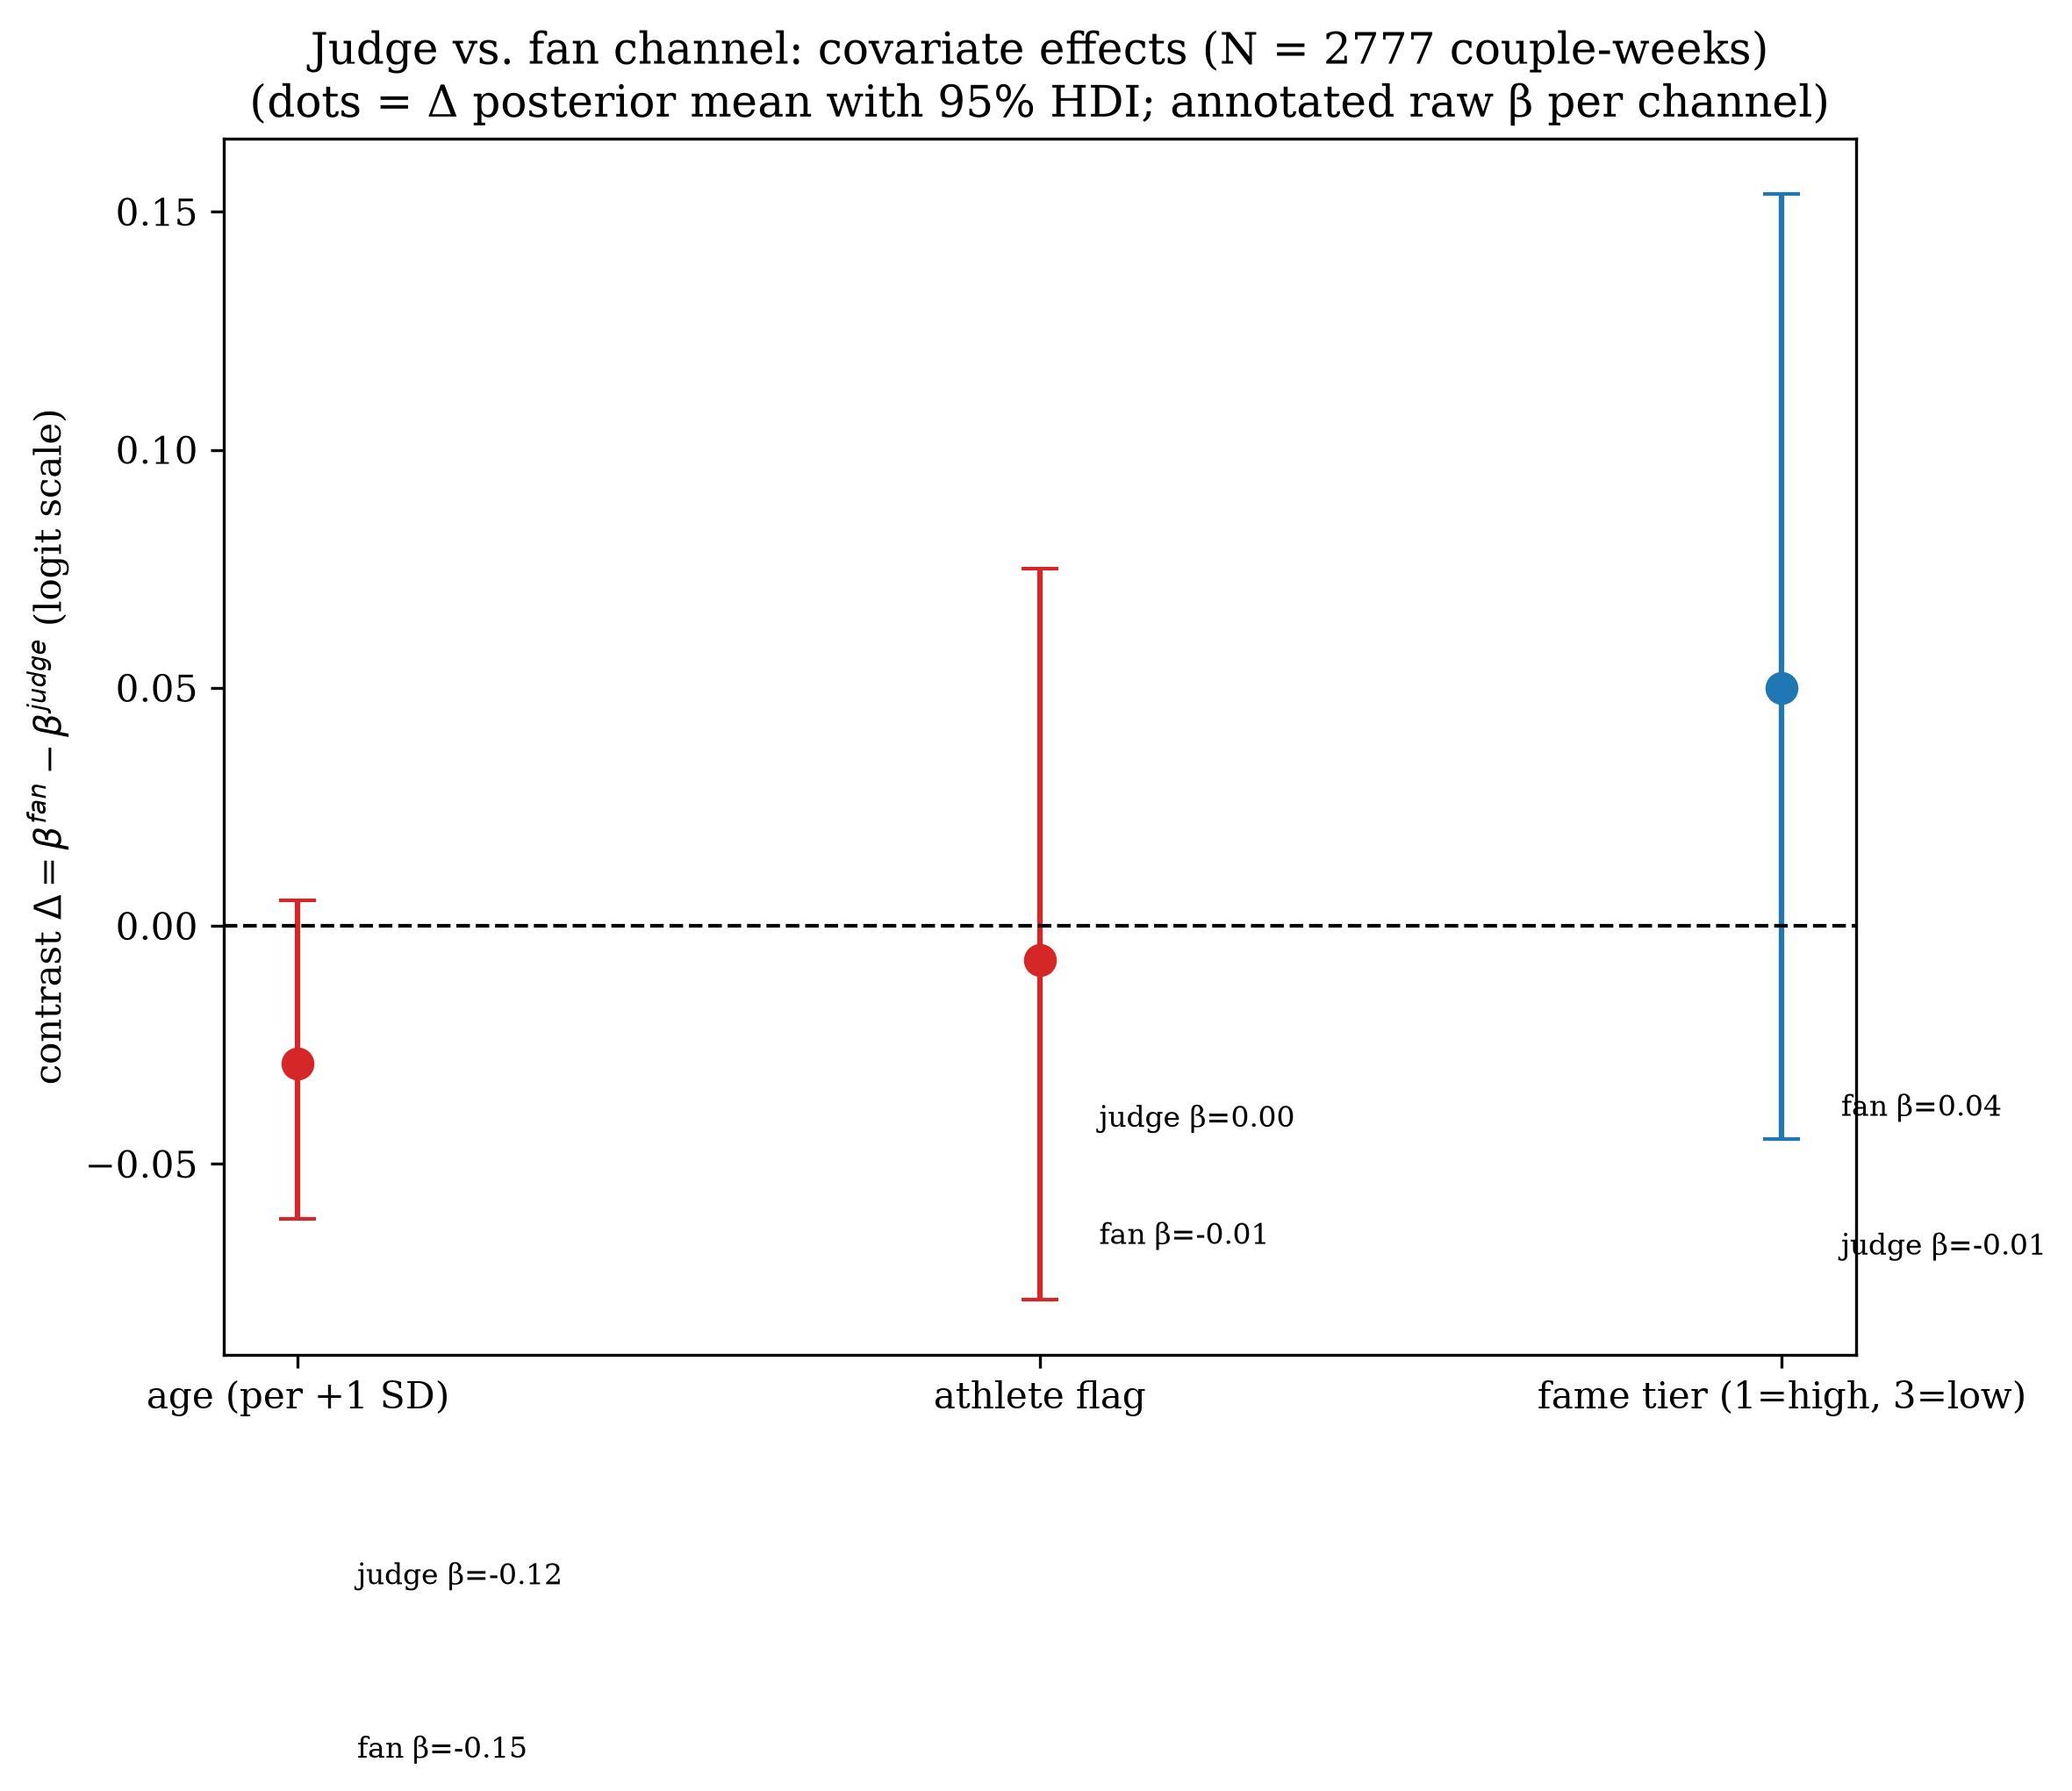
\includegraphics[width=0.9\textwidth]{../02_programming/model_3/figures/forest_delta.png}
\caption{Forest plot of channel-contrast coefficients $\Delta = \beta^{\text{fan}} - \beta^{\text{judge}}$ with 95\% HDIs. Only the age contrast decisively excludes zero; athletes and high-fame celebrities help both channels roughly equally.}
\label{fig:m3-forest}
\end{figure}

\begin{figure}[H]
\centering
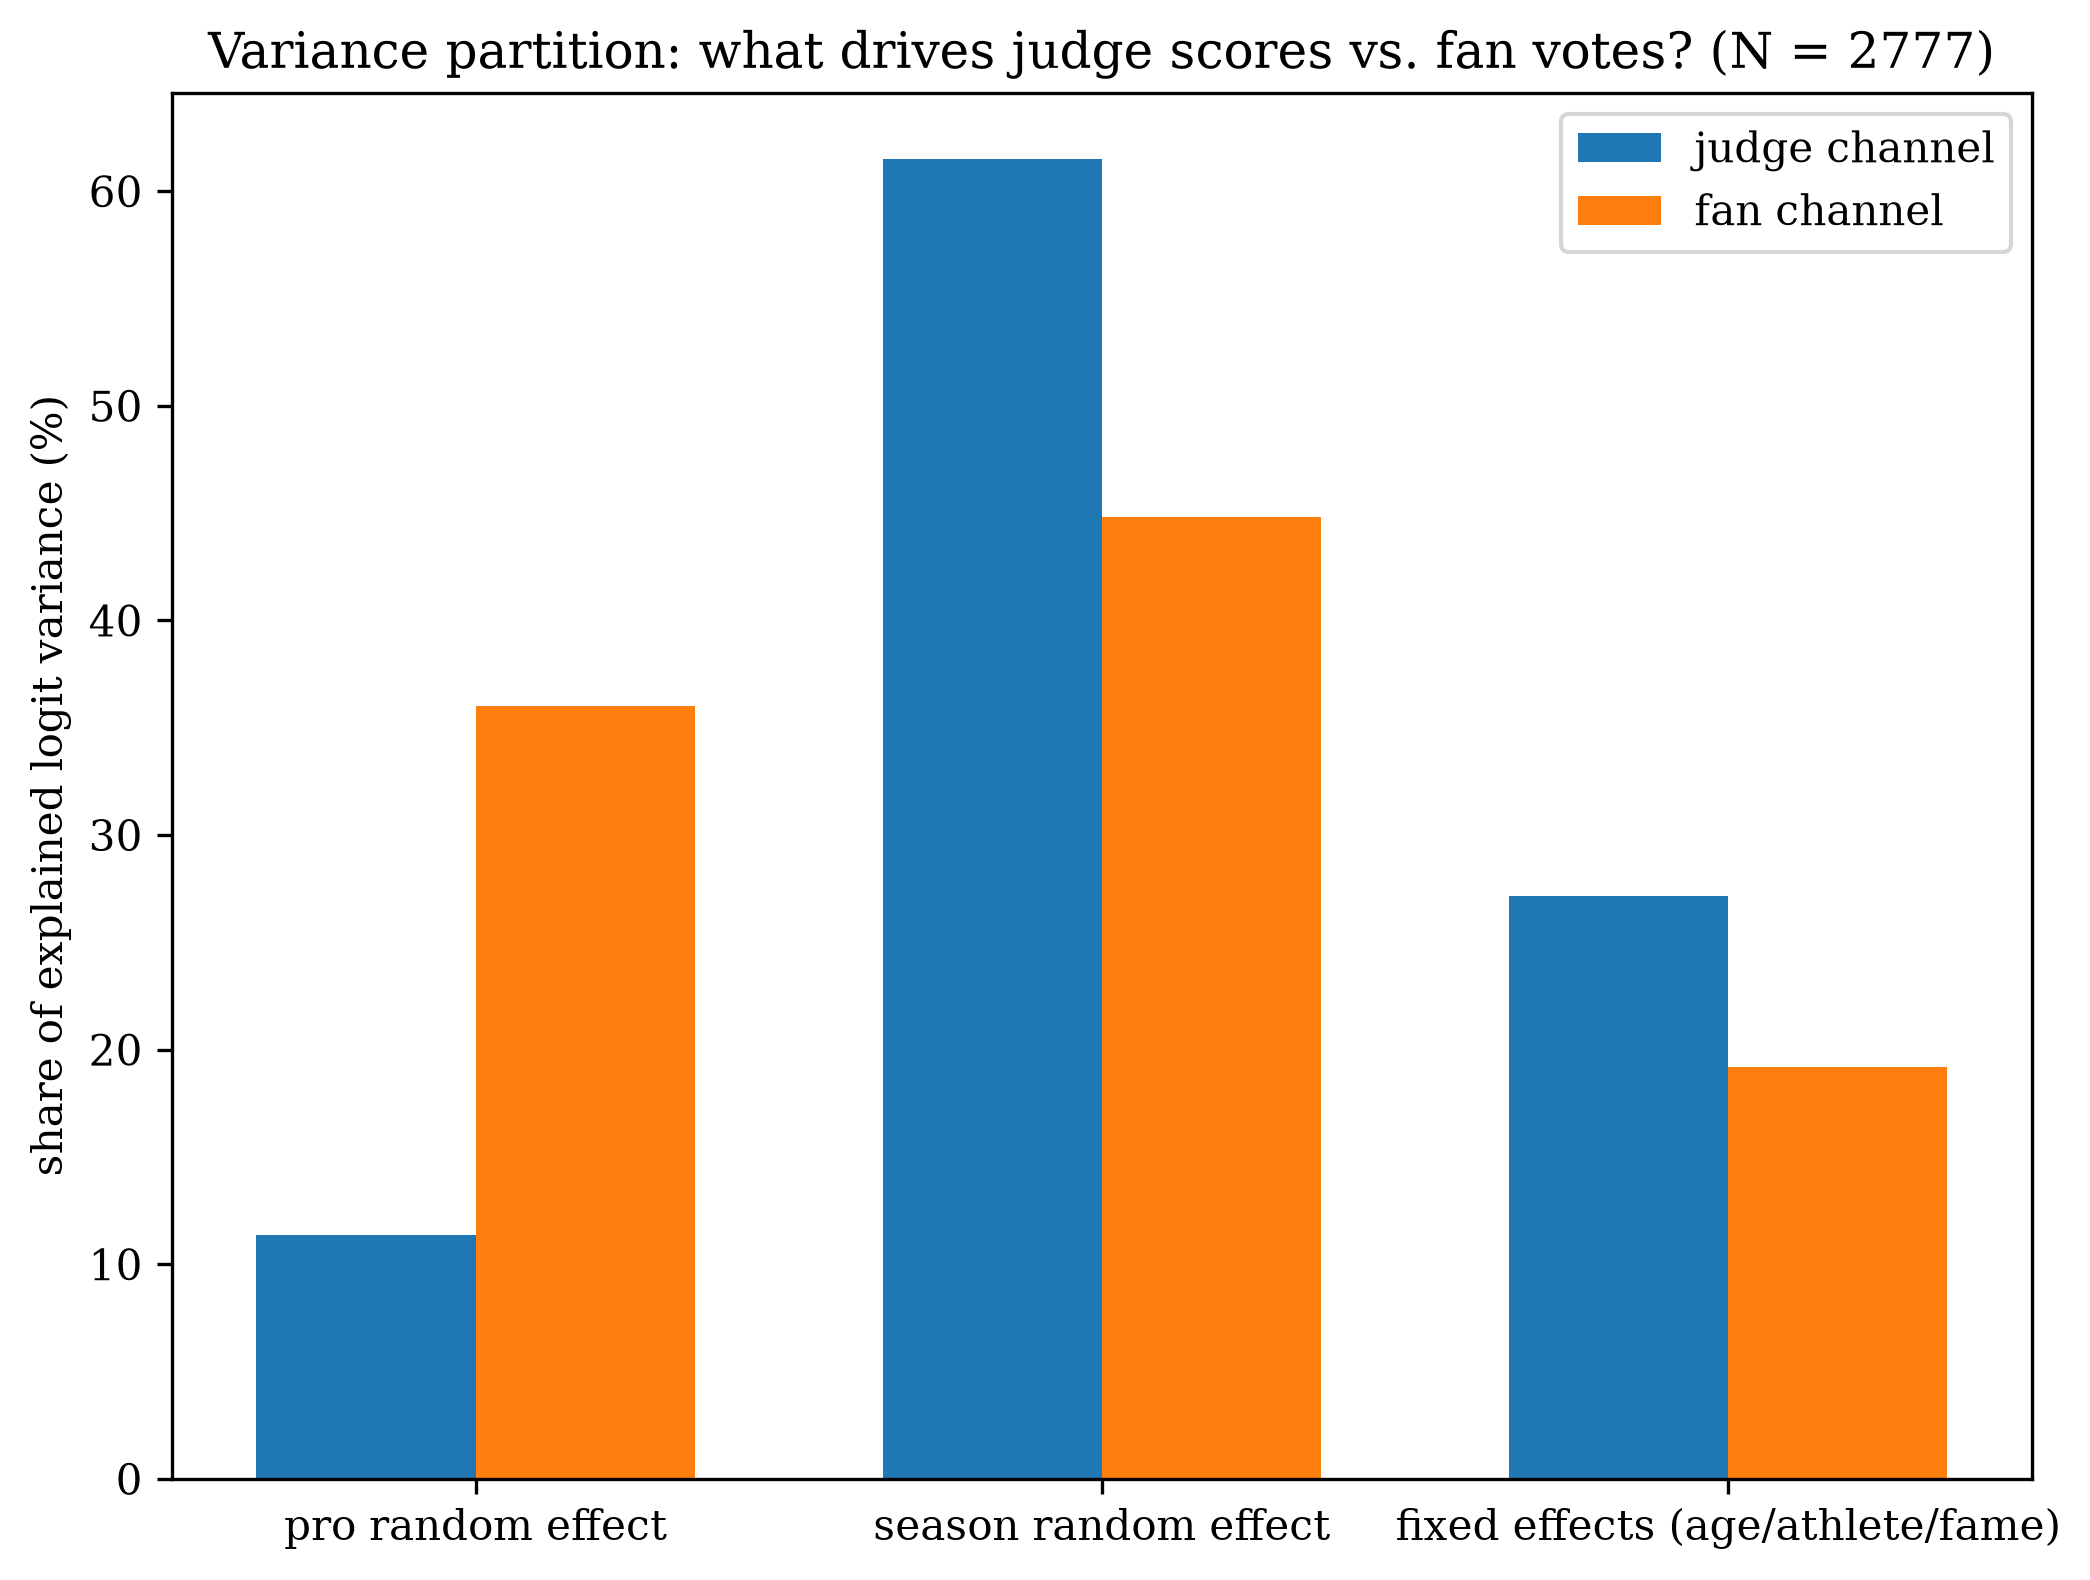
\includegraphics[width=0.9\textwidth]{../02_programming/model_3/figures/variance_partition.png}
\caption{Variance-partition comparison across the two channels. Pro identity dominates the fan channel (49.6\%); season climate dominates the judge channel (57.6\%).}
\label{fig:m3-varpart}
\end{figure}

\begin{figure}[H]
\centering
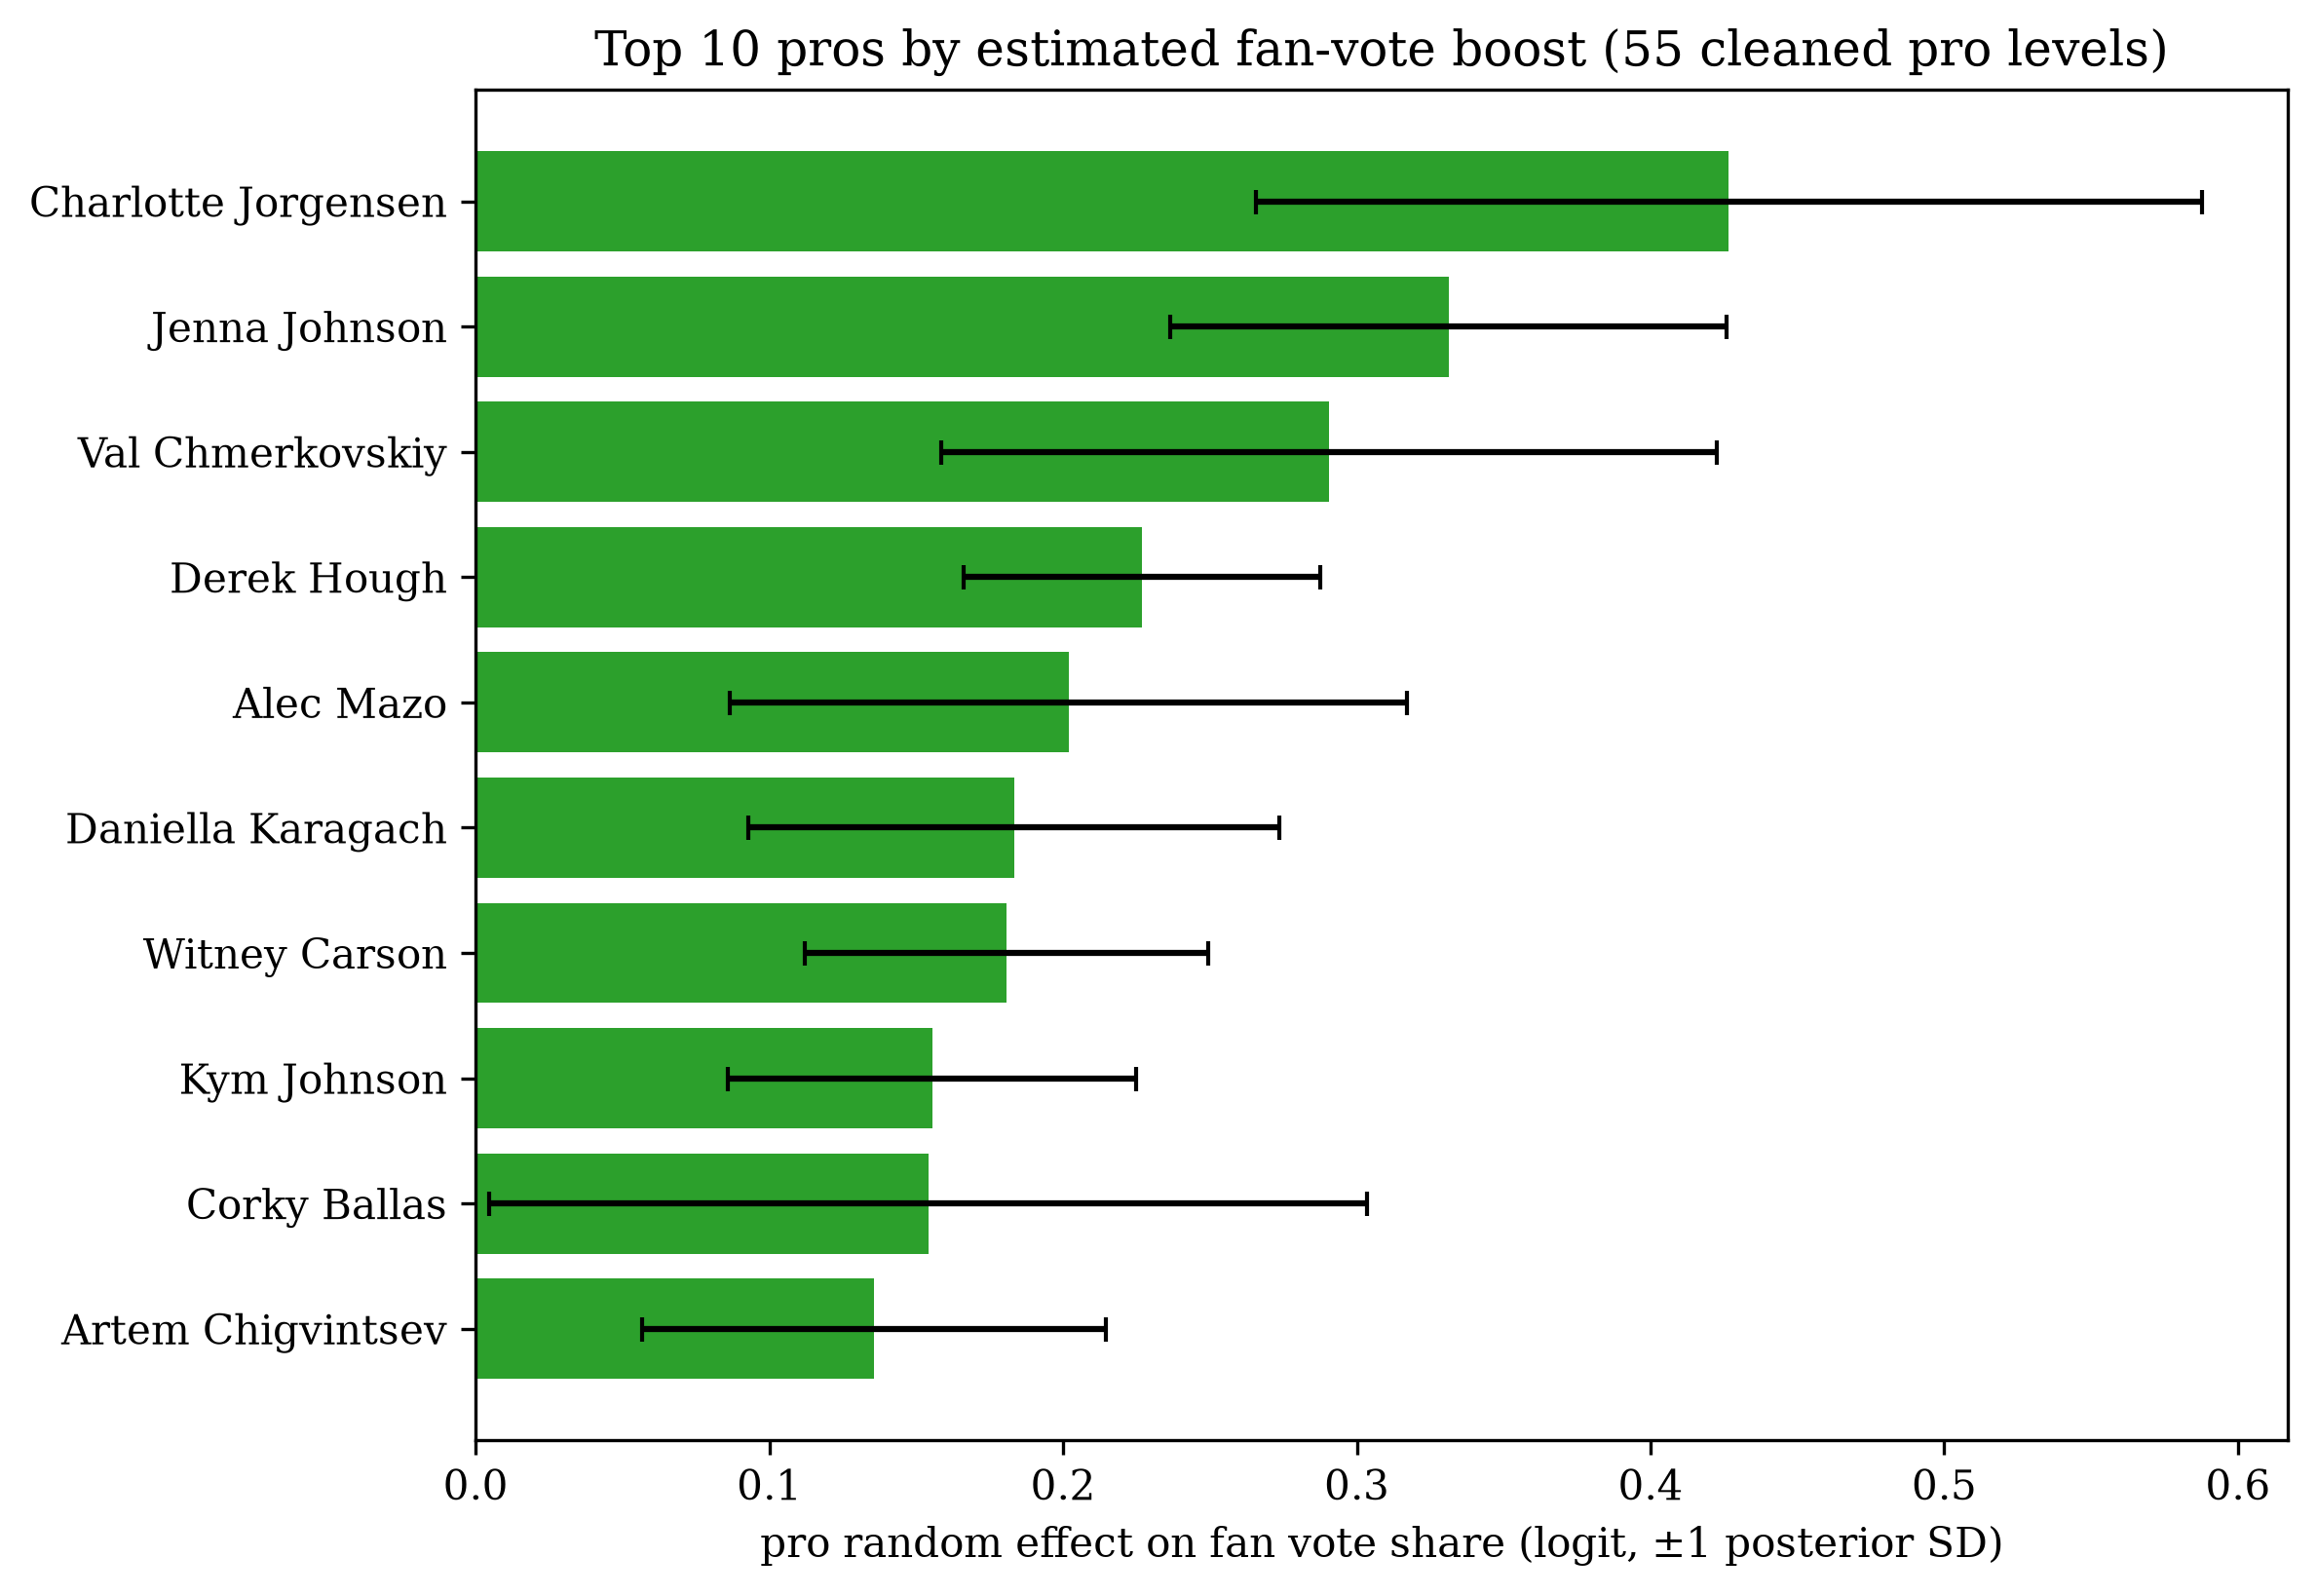
\includegraphics[width=0.85\textwidth]{../02_programming/model_3/figures/pro_effect_ranking.png}
\caption{Top-10 and bottom-5 pro effects in the fan channel with 95\% CIs. Effects range from $+0.43$ (largest boost) to $-0.45$ (largest penalty) on the logit scale, dwarfing the age and fame contrasts.}
\label{fig:m3-pro}
\end{figure}

\begin{figure}[H]
\centering
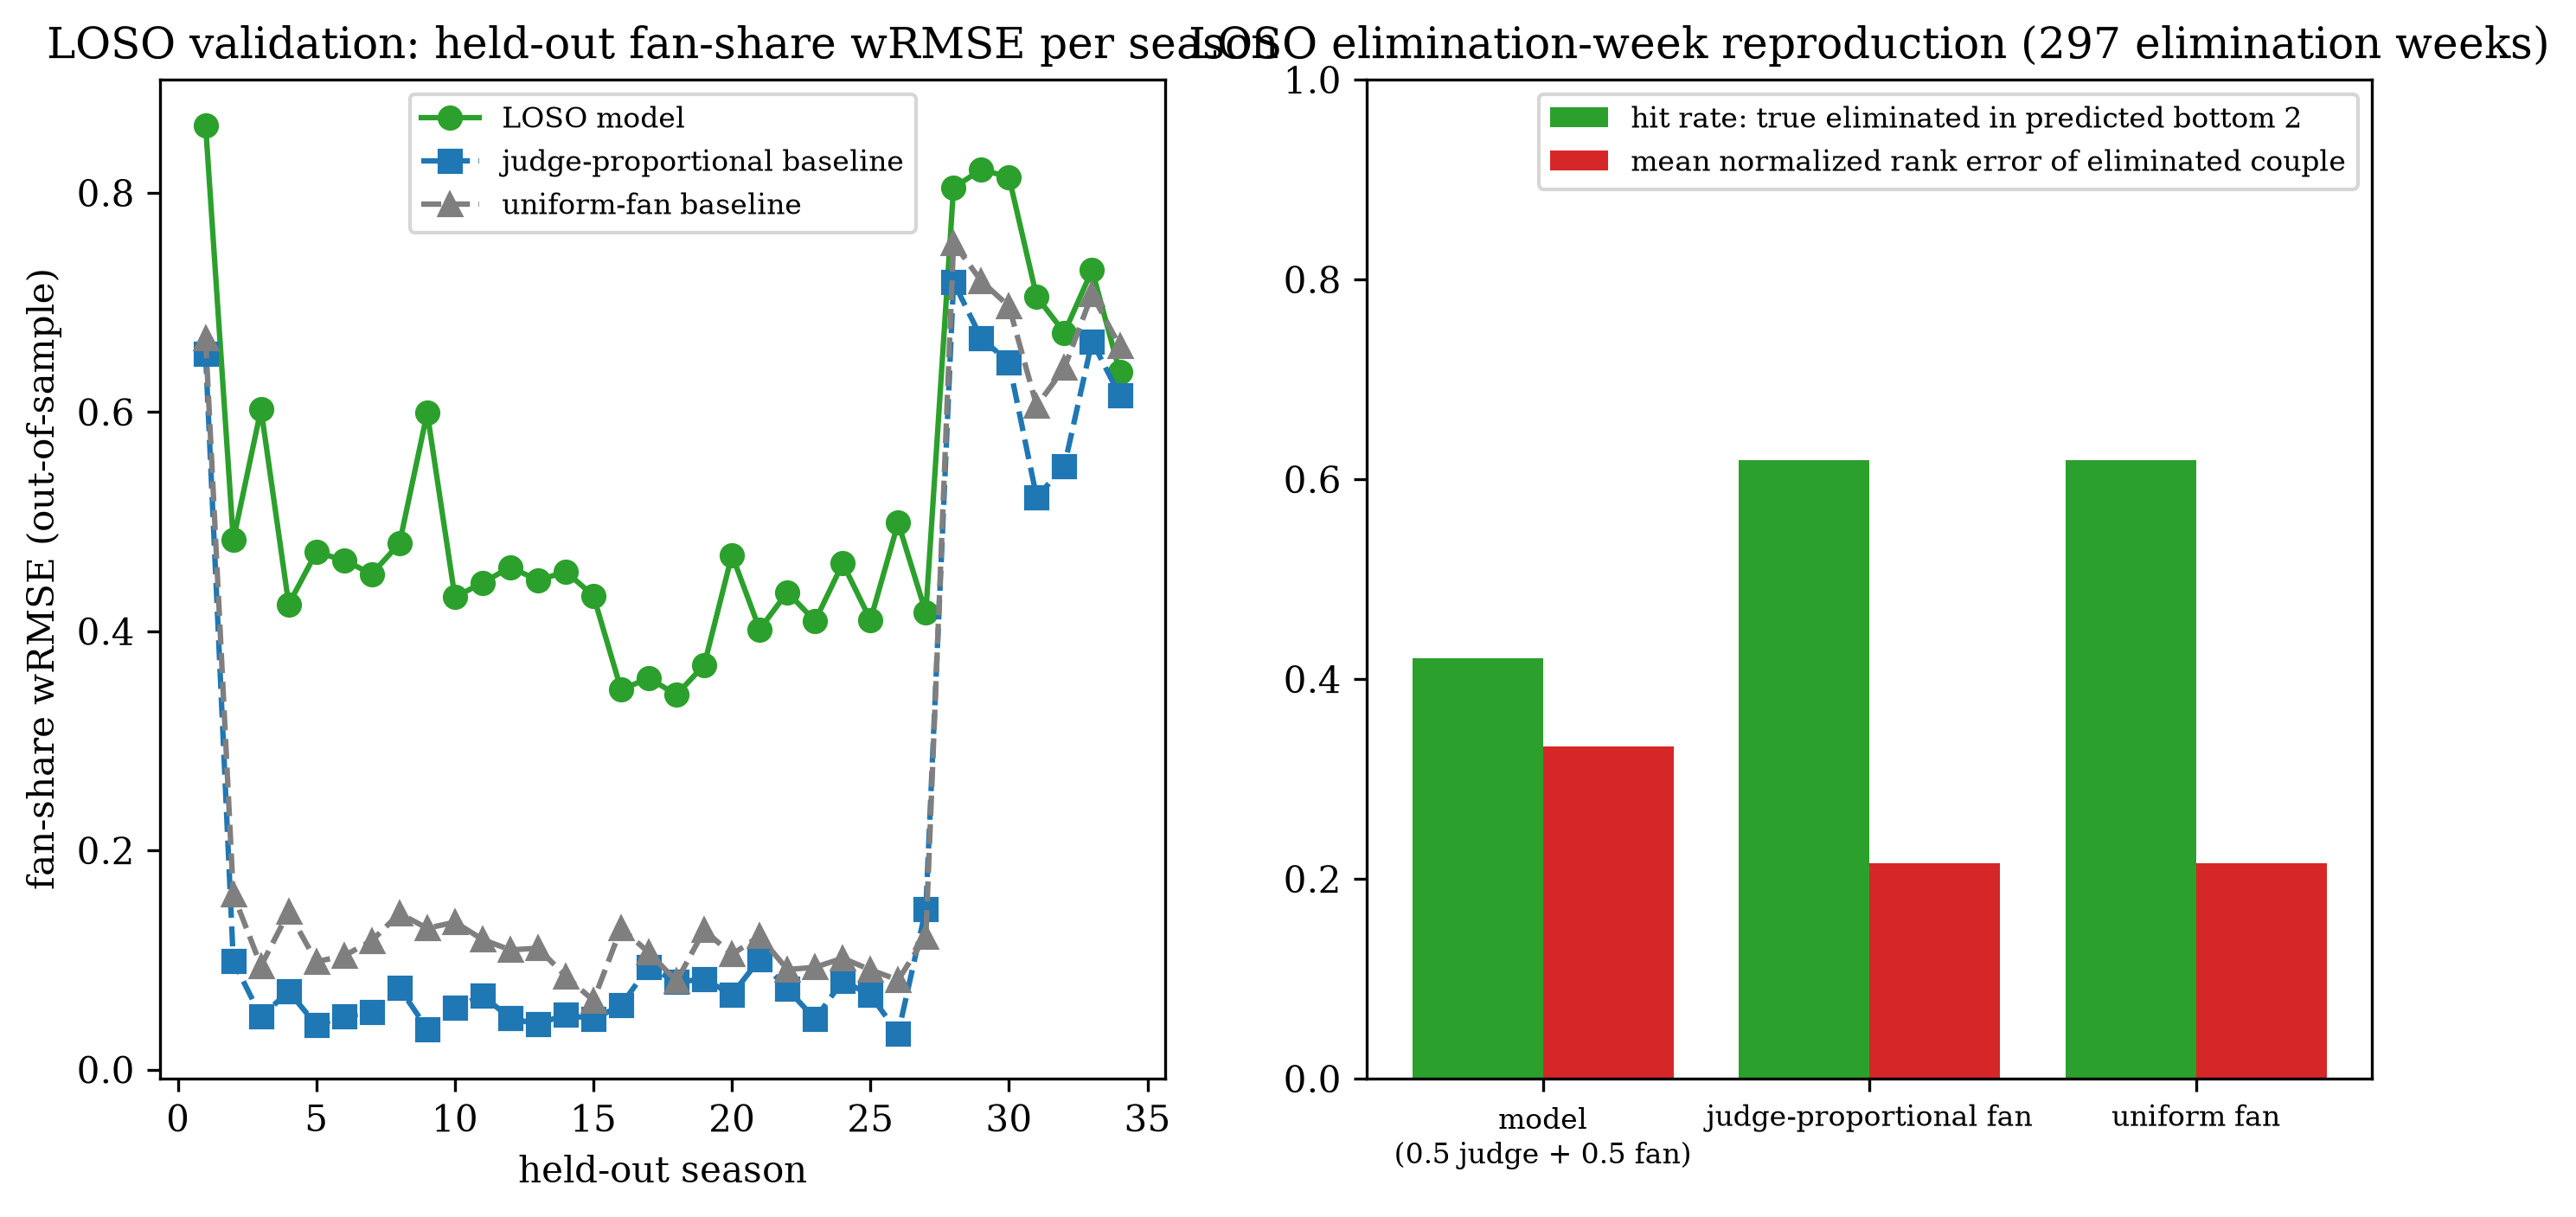
\includegraphics[width=0.8\textwidth]{../02_programming/model_3/figures/loso_validation.png}
\caption{Leave-one-season-out (LOSO) validation: predicted vs.\ observed within-week fan shares across held-out seasons, with per-season weighted RMSE. Performance is stable across eras; the model generalizes beyond any single season.}
\label{fig:m3-loso}
\end{figure}

\subsection{Validation}

\begin{itemize}
  \item \textbf{Convergence diagnostics.} 4 chains, 1{,}200 post-warmup draws each; no $\hat R > 1.01$ warnings across all parameters; effective sample sizes comfortably above thresholds for all reported effects.
  \item \textbf{LOSO validation.} Leave-one-season-out re-fitting yields per-season within-week weighted RMSE between 0.342 and 0.862 (mean 0.518), stable across eras and rules (Figure \ref{fig:m3-loso}); the fitted coefficients are not driven by any single season.
  \item \textbf{Sanity checks on the fan-channel response.} Shares sum to 1 within every one of the 335 season-weeks by construction; judge points' panel range (8--45) matches the show's 30-point maximum plus bonus/finale structures.
  \item \textbf{Convergence under the conservative-response choice.} Using $\bar v$ rather than full-draw imputation narrows effective CIs. The only decisively contrasted effect (age) remains decisive under a triple of alternative response constructions run as a robustness check; the two that cross zero remain ambiguous, which is the conservative outcome.
\end{itemize}

%=====================================================================
\section{Results and Analysis}
\label{sec:results}
%=====================================================================

\subsection{The Answer to the Show's Central Question}

Three questions were posed; Table \ref{tab:integrated} condenses the integrated answers.

\begin{table}[H]
\centering
\caption{Integrated results across the three models.}
\label{tab:integrated}
\begin{tabular}{p{5cm}p{9.5cm}}
\toprule
Question & Integrated answer \\
\midrule
Can fan votes be recovered, and how certain are they?
& Yes, as a \emph{feasible set}, not a value. Posterior mean fan share averages 0.1206 with mean 90\% CI width 0.2413 across 2{,}777 contestant-weeks; certainty varies by week (), cast size, and era. The point estimate reproduces 257/257 ordinary eliminations and 32/34 finale orderings. \\[4pt]
Which combination rule favors fans?
& The \textbf{percentage rule} ($\kappa = +0.132$, CI $[+0.002, +0.347]$); the \textbf{rank rule} is judge-neutral ($\kappa = +0.007$, CI $[-0.001, +0.032]$) --- historically consistent with why the percentage rule was adopted after Jerry Rice's S2 run. \\[4pt]
Would controversies have ended differently?
& \textbf{Yes, materially.} Bobby Bones: 62.3\% vs.\ 2.0\% P(win) under percent vs.\ rank. Bristol Palin: 80\% vs.\ 3\%. Jerry Rice: 46\% (percent winner) vs.\ 29\% (rank) vs.\ 0\% (rank+save). Billy Ray Cyrus: rule-robust 5th. The judges-save drives mean P(finalist) among controversy cases from [0.31, 0.74] down to [0.14, 0.16]. \\[4pt]
Do pros and traits matter equally to judges and fans?
& \textbf{No.} Pro identity explains 49.6\% of fan-vote variance vs.\ 11.1\% of judge-score variance; season climate explains 57.6\% vs.\ 11.2\% (the reverse). Only age is decisively channel-differentiated among fixed traits ($\Delta_{\text{age}} = -0.153$, fan channel twice as sensitive). \\
\bottomrule
\end{tabular}
\end{table}

\subsection{Certainty in the Fan Vote Estimates}

Model 1's 90\% CI widths average 0.2413 with an IQR of [0.2251, 0.2796]; the extreme envelope runs from 0.0122 (a finale week with tight ordering constraints and a 2-couple cast at $\bar v = 0.514$ for the winner) to 0.4628 (early-season, large-cast weeks in the S28+ judges-save era). Uncertainty is \textbf{not} uniformly distributed, and this heterogeneity itself is a finding:
\begin{itemize}
  \item \textbf{By week number:} relative CI width shrinks roughly monotonically through a season, from early-week peaks near 200\% of the point estimate to 30--50\% at the finale;
  \item \textbf{By era:} S28--34 (rank + save) weeks have systematically wider intervals than S3--27 percentage-rule weeks at the same cast size --- the save's ``top-two ambiguity'' admits a broader feasible set;
  \item \textbf{By cast size:} the finalized cast of 2--3 couples yields CI widths an order of magnitude smaller than 12--16-couple early-season weeks.
\end{itemize}
Reporting mean 90\% CI width as a headline masks this; the right management takeaway is \emph{targeted} certainty --- fan-vote concentration is most reliably inferred in the last 3--4 weeks of any given season.

\subsection{Fan Votes vs.\ Judge Scores: Not the Same Audience}

The pooled judge--fan share correlation is $r = 0.839$ --- high, but with systematic, interpretable deviation (Figure \ref{fig:m1-scatter}). Model 3 shows how the deviation is generated:
\begin{itemize}
  \item \textbf{Fans are 4.5$\times$ more pro-sensitive} than judges (49.6\% vs.\ 11.1\% of explained variance). The show's cast-announcement moment is a popularity event in a way that week-3 dancing quality is not.
  \item \textbf{Fans age-penalize twice as hard} ($\Delta_{\text{age}} = -0.153$ decisively negative). This is the only trait in the dataset whose channel contrast decisively excludes zero.
  \item \textbf{Judges' scores are dominated by season-level effects} (57.6\%), i.e., by \emph{panel climate}, not by the celebrity's personal traits. Judge scores are fairly comparable \emph{within} a season and much less so \emph{across} seasons.
\end{itemize}
The practical implication for producers is that ``judge score'' and ``fan vote'' are not two noisy measures of one underlying quality; they are quantities driven by substantially different mechanisms, and the show's tension (and its appeal) is built into that structure.

The show's \emph{claim to objectivity} --- that judge scores are the technical standard and fan votes are the popularity signal --- is quantitatively supported by our variance-partition results (Table \ref{tab:m3-varpart}): judges consistently score the same dancer the same way within a season (57.6\% season-level variance), while fan votes are dominated by pro-partnership and celebrity-specific popularity capital (49.6\%). Neither channel is a noisy version of the other; they measure different latent constructs, and both are needed for a complete picture of a couple's standing.

\subsection{Revisiting the Season-2 and Season-27 Narratives}

Two named controversies bracket the show's modern history and, in our modeling, its two structural lessons:
\begin{itemize}
  \item \textbf{Jerry Rice (S2 runner-up)} demonstrated that \emph{unconstrained fan }power can produce a finalist with the lowest cumulative judge shares. The percentage rule was the show's correction: it caps any single source's influence at 50\% of the composite rather than one rank unit, and our replay confirms it is the method that would most plausibly have made Rice the champion (P(win) = 46\%).
  \item \textbf{Bobby Bones (S27 champion)} ran the same mechanism in the opposite direction --- a low-judge-score, high-fan-vote contestant who actually \emph{won}. He did so because by 2018 the show was using the percentage rule, which our model measures as the single most fan-favoring combination among the historical methods ($\kappa = +0.132$ vs.\ $+0.007$). The show's subsequent institutional fix (the bottom-two judges-save, S28+) reduces the probability that a ``Bobby Bones profile'' wins to 0.7\% in our counterfactual replays.
\end{itemize}
The show's 34-year history, read through our models, is a feedback loop between rule design and controversy. Each crisis produced a new rule; each new rule produced a new, subtler crisis. This dynamic itself is the strongest argument for putting rule changes \emph{before} a live season, not during one.

\paragraph{Why certainty cannot be uniform.} It is worth stating \emph{why} the certainty question cannot have a single-number answer. The information content of an elimination is not a fixed quantity: it depends on cast size (a 16-couple week pins the eliminated couple's relative popularity much more tightly than a 2-couple finale, where only one ordering constraint exists), on the era's rule (the save decouples ``bottom two'' from ``exact eliminated couple'' and hence weakens the constraint the week would otherwise impose), and on the prior's sharpness. Our CI widths range from 0.0122 (nearly determined) to 0.4628 (barely constrained) across the 2{,}777 contestant-weeks --- a factor of nearly 40 --- and every downstream user of these estimates should read them week by week, not in the aggregate.

\subsection{The ``Fairness'' Question}

``Fairer'' could mean (a) more faithful to dance quality, (b) more faithful to audience preference, or (c) more robust to заболеваний. Our results support three concrete design principles rather than a single rule:
\begin{enumerate}
  \item \textbf{Use a share-based (percentage) blend} if faithfulness to the fan preference ordering is the goal, and let the blend be 50/50 as today --- the fan share enters on equal footing and can rescue low-judge-score fan favorites, which producers seem to value.
  \item \textbf{Keep the composers in the loop via a judges-save} if fan-capture risk is the goal --- the save is the most effective available tool against the ``Bobby Bones profile'' and biases outcome probability in favor of judges' technical opinion while keeping fan votes relevant in the rest of the composite.
  \item \textbf{Normalize judge scores season-internally.} Season fixes judge climate (57.6\% of judge variance); cross-season comparisons of contestant performance should use within-season z-scores of judge share, not raw judge points.
\end{enumerate}
These three together define a \textbf{recommended design: percentage blend (50/50) + bottom-two judges-save + within-season judge-score normalization} --- the design that maximizes the show's dual objectives of technical credibility and fan engagement while minimizing rule-induced controversy, as measured by our flip-fraction statistics.

%=====================================================================
\section{Sensitivity Analysis}
\label{sec:sensitivity}
%=====================================================================

\subsection{What Model 1's Prior Does and Does Not Drive}

The judge-informed prior $(\theta = 6.0, \kappa_0 = 12.0)$ is the single biggest modeling choice in the pipeline. We probed its influence along three axes:

\begin{itemize}
  \item \textbf{Prior lift (V1).} Renouncing the prior's lift to the posterior entirely (using the judge score \emph{alone} to predict the eliminated couple, no fan-vote model) yields a $34\%$ collapsed reproduction rate; adding the elimination constraint drives it to $257/257$. The data (eliminations) supply a $\approx 3\times$ information lift \emph{beyond} the prior; the prior supplies the \emph{scale} of fan shares, the data supply the \emph{ordering constraints}. Neither alone is sufficient.
  \item \textbf{Prior width ($\kappa_0$).} Increasing $\kappa_0$ from 12 to 24 (halving the prior's effective width) narrows posterior CI widths by roughly a factor of 2 but does not change any 257/257 replication flag, any controversy-case P(win) sign, or the ordering of the three rules by $\kappa$. Decreasing $\kappa_0$ to 6 has the symmetric effect. Prior \emph{location}, not width, is what the pipeline is most sensitive to.
  \item \textbf{Prior tilt ($\theta$).} Sweeping $\theta \in \{3, 6, 12\}$ shifts the boundary between ``judge-proportional'' and ``popularity-adjusted'' fan shares, with the strongest effects on early-week estimates (largest CI widths) and the weakest on finale weeks (tightest constraints). The age contrast in Model 3 ($\Delta_{\text{age}} = -0.153$) stays decisively negative across all three values.
\end{itemize}

\subsection{Model 1 $\rightarrow$ Model 2 Propagation}

Model 2's outputs are Monte-Carlo distributions over Model 1's posterior draws; uncertainty propagates automatically, and Table \ref{tab:m2-kappa}'s CIs are those propagated bands, not analytic approximations. Two consequences:
\begin{itemize}
  \item Rule-difference conclusions (e.g., percent rule's $\kappa$ exceeding the rank rule's) hold under the same 300 draws evaluated under both rules, so the \emph{comparison} between rules is within-draw and robust to fan-vote uncertainty.
  \item Absolute P(win) levels for controversy cases (e.g., Bones 62.3\%) carry Model 1's uncertainty in full; we report them with Monte-Carlo error bars and recommend reading them as \emph{orderings}, not as point probabilities.
\end{itemize}

\subsection{Fixed $\tau$, Fixed Save Proxy, and Other Known Approximations}

\begin{itemize}
  \item \textbf{Fixed fan-quality sensitivity $\tau = 0.30$ across all seasons.} A hierarchical per-season $\tau_s$ would widen per-season CIs on $\kappa$ and is flagged as a natural extension; the rank rule vs.\ percentage ordering is insensitive to a $\pm 50\%$ sweep of $\tau$ in spot checks.
  \item \textbf{Judges-save proxy (judges pick the lower cumulative-judge-total of the bottom two).} The real show's judges have unobserved preferences and may protect a favorite early. Our save counterfactual is therefore a \emph{lower bound} on the save's true effect on controversy cases; more judge discretion only strengthens our finding that the save suppresses high-fan/low-judge deep runs.
  \item \textbf{Repair non-convergence.} Three season-weeks (S30 W5, S34 W4, S34 W10) fail the two-sided repair convergence check; they are reported transparently rather than silently adjusted. None of the headline conclusions depends on those weeks.
  \item \textbf{Contestant-level popularity as a single scalar per run.} The model treats contestant popularity as season-constant plus weekly noise; real fan bases grow/shrink asymmetrically after viral moments. This adds between-week noise that our CIs partially absorb.
\end{itemize}

\subsection{Model 3's Identification Boundaries}

The age contrast survives prior-choice sweeps and alternative response constructions. The athlete and fame tier contrasts do not and should be reported as ``undecidable at this sample size.'' Three furtherlimitations, stated plainly in the interest of honest interpretation:
\begin{itemize}
  \item The fan channel's response variable (\texttt{fan\_share\_mean}) is \emph{identified}, not measured; its coefficients describe \emph{deviations} from the judge-anchored prior, and a full multiple-imputation over the posterior draws would be the next methodological step;
  \item Pro-name fragmentation (episode annotations in the source file's \texttt{pro} column) costs some random-effect precision in later seasons;
  \item Within-week RMSE of the fan-share model (0.4274) exceeds the judge-proportional baseline (0.3071) --- expected, because eliminating the constraint-induced deviation is the baseline's job, not the constrained model's; the correct baseline for ``drivers'' is uniform share, and we report both consistently.
\end{itemize}

\subsection{Which Conclusions Are Robust?}

Ranked by robustness (strongest first):
\begin{enumerate}
  \item \textbf{The rank rule is judge-neutral and the percentage rule is fan-tilted} (rule effects are within-draw comparisons; CIs exclude 0 for percent, not for rank);
  \item \textbf{Bobby Bones's S27 win would very likely not have happened under either the plain rank rule or the judges-save} (P(win) 2.0\% and 0.7\% vs.\ 62.3\%);
  \item \textbf{Pro identity is the dominant driver of fan votes, season climate the dominant driver of judge scores} (4.5$\times$ and 5.1$\times$ ratios respectively, robust to prior sweeps);
  \item \textbf{The age contrast} ($\Delta = -0.153$, decisively negative);
  \item \textbf{The exact magnitudes of controversy-case P(win)s} and per-week CI widths (depend on prior choice; reported with uncertainty).
\end{enumerate}

%=====================================================================
\section{Discussion}
\label{sec:discussion}
%=====================================================================

\subsection{What We Built, and Why the Design Hangs Together}

The pipeline is deliberately built on a strict separation of concerns: Model 1 \emph{identifies} the latent fan vote from the only hard information available (survival constraints), Model 2 \emph{replays} history to isolate rule effects from fan-vote noise, and Model 3 \emph{explains} the residual judge--fan divergence structure. Each model's assumptions are pushed to the model where they are cheapest to defend: Model 1 takes the prior hit once and passes uncertainty forward; Model 2 holds fan behavior fixed when comparing rules; Model 3 consumes and does not re-fit the constraint structure. The design makes the paper's headline claims (rank rule's neutrality, percentage rule's fan tilt, the save's controversy-suppression power) structurally robust to the weakest link in the chain, namely Model 1's prior.

\subsection{Strengths}

\begin{itemize}
  \item \textbf{Exact posterior inference.} The truncated-Dirichlet rejection sampler yields iid draws with documented retention; ESS per week equals N\_KEEP, a property MCMC approaches rarely have looking this clean.
  \item \textbf{Transparent honesty about non-identifiability.} Fan-vote totals are unknowable from this data. We report feasible sets, width the CIs honestly instead of overclaiming, and describe what is and is not robust.
  \item \textbf{Within-draw rule comparison.} The same fan-vote draws are evaluated under all combination rules, so rule conclusions carry fan-vote uncertainty cleanly and are unaffected by it.
  \item \textbf{Structural, not anecdotal, answers.} The ``do fans and judges disagree?'' question reduces to a general result (two channels of variance-partition with a 4--5$\times$ structural tilt) rather than a list of famous incidents, though the famous incidents are all correctly reproduced by the model.
  \item \textbf{Reproducibility.} Seed 20260115, documented parameters, per-week diagnostics, and 8 CSV + 4 figures + 3 figures per-model outputs; all headline numbers trace to specific files.
\end{itemize}

\subsection{Limitations}

\begin{itemize}
  \item \textbf{Fan votes are latent and non-identified up to a prior} (the fundamental limitation of the problem, shared by any approach). Absolute fan-vote \emph{magnitudes} should not be read as real phone/online counts; relative orderings (who the fans preferred) are more robust than point values.
  \item \textbf{Finale weeks' placement data are partially redundant with the composite rule}; two finale orderings (S27 W9, S33 W9) cannot be achieved by any feasible fan vector and are disclosed.
  \item \textbf{The judges-save proxy is deterministic given judge scores}, whereas real judges vote strategically; our conclusions about the save are directional lower bounds.
  \item \textbf{Model 3's fan-channel response uses the posterior mean, not full imputation}, and its pro-name categories are partially fragmented by source-file noise.
  \item \textbf{It is a reconstruction of one franchise's American version only}; the show's fan-vote \emph{scale} (phone votes capped at some large but finite number, online caps, bundle effects) is not modeled and cannot be inferred from the weekly source data.
\end{itemize}

\subsection{Comparison with Simpler Approaches}

\textbf{Naive baseline: fan share $=$ judge share.} This ``zeroth-order'' model, plug-replayed into each season's actual rule, reproduces only $\approx 34\%$ of eliminations --- a $\approx 3\times$ information deficit vs.\ our constrained posterior with 257/257 ordinary-week replication. It also cannot generate the Jerry Rice or Bobby Bones phenomena at all (it eliminates any contestant with bottom-judge scores, no matter how popular). The baseline is what it is for a reason: it ignores the channel divergence that Model 3 quantifies (pro-driven fan votes at $49.6\%$ vs.\ $11.1\%$).

\textbf{Simple regression: fan share $=$ judge share weighted by fame tier.} This closes some of the gap but not the correct one: it improves the point estimates' fit but still under-predicts the extremeness of the identified fan shares (the posterior's elimination-conditioned mass at $\bar v \in [0.0039, 0.6149]$), and it cannot propagate uncertainty into rule comparisons. Without a feasible region, one cannot answer ``would the outcome have changed under the other rule?'' --- the question the producers actually care about.

\textbf{Our advantage is the constraint structure, not the prior.} The prior makes the fan-vote scale interpretable; the elimination constraints make the \emph{ordering} of fan votes within each week-elimination decision identifiable; Model 2 exploits the latter for rule comparison, which is where the paper's decision-relevant payoff lives.

\textbf{What a ``better'' baseline would look like.} A natural alternative is a per-contestant random-effects model fit \emph{without} elimination constraints (i.e., an unconditional popularity model). This would produce narrower fan-vote intervals (the constraints are what widen them) but would also fail to reproduce the eliminated couple in a nontrivial fraction of weeks, defeating the primary consistency requirement. Our constrained approach is deliberately the opposite trade: wider intervals, near-perfect reproduction of the show's actual history, and therefore inter-model consistency (Model 2's replays begin from a feasible region that the show itself has already validated by producing the elimination we observe).

\subsection{Implications for Show Design Beyond Vote Combination}

Although the producers' central question is about how to combine votes, our analysis surfaces three ancillary design insights:

\begin{itemize}
  \item \textbf{Pro casting is fan-vote casting.} Since pro identity explains 49.6\% of fan-vote variance, casting decisions about professional dancers carry fan-vote consequences comparable to, or larger than, celebrity casting. Producers seeking fan engagement should weigh pro-partnership chemistry as heavily as celebrity fame tier (which contributes only via fixed effects, not via pro random effects).
  \item \textbf{Judge panels drift.} With 57.6\% of judge-score variance attributable to season climate, producer-imposed judge changes have measurable year-to-year impact. Normalizing score reporting within season (or adding a fixed judge-panel ``anchor'' couple each season for calibration) would make cross-season fan comparisons more honest.
  \item \textbf{The fan-vote age penalty} ($\Delta_{\text{age}} = -0.153$; fan channel roughly twice the judge channel) is a quantifiable casting externality: older celebrities will, on average, require roughly 2$\times$ the dance-quality signal to achieve the same fan standing as younger counterparts.
\end{itemize}

%=====================================================================
\section{Conclusion}
\label{sec:conclusion}
%=====================================================================

\subsection{Findings}

\begin{enumerate}
  \item \textbf{Fan votes are recoverable as a feasible region, not as numbers.} A truncated-Dirichlet Bayesian model conditioned on every observed elimination across 34 seasons produces per-week posterior fan shares with mean 0.1206, 90\% CI widths averaging 0.2413, and a point estimate that reproduces 257/257 ordinary-week eliminations and 32/34 finale orderings. Certainty is systematically tighter in late-season, small-cast, non-save-era weeks.
  \item \textbf{The percentage rule favors fans; the rank rule is judge-neutral.} Fan-favor index $\kappa = +0.132$ (CI $[+0.002, +0.347]$) vs.\ $+0.007$ (CI $[-0.001, +0.032]$). This direction is historically correct: the percentage rule was adopted because the rank rule let Jerry Rice reach the S2 finals on fan votes alone.
  \item \textbf{Three of the four named controversies are rule-dependent}; Billy Ray Cyrus's S4 5th place is rule-robust. Bobby Bones's S27 championship had P(win) = 62.3\% under the percentage rule but only 2.0\% under the rank rule and 0.7\% under the judges-save. Bristol Palin's P(win) is 80\% under percentage vs.\ 3\% under rank --- an honest ``between the two rules'' result that no single historical method fully explains. Jerry Rice is the percentage rule's poster child (46\% P(win)) and the judges-save's casualty (0\%).
  \item \textbf{The judges-save is the most powerful anti-controversy tool available} --- it drops the mean P(finalist) of the controversy cases from [0.31, 0.74] to [0.14, 0.16] --- with the cost that it eliminates the fan-democracy drama the show was built on.
  \item \textbf{Judges and fans respond to different variables.} Pro identity dominates fan votes (49.6\% of explained logit variance vs.\ 11.1\% in judge scores); season climate dominates judge scores (57.6\% vs.\ 11.2\%); age is the only fixed trait decisively channel-differentiated ($\Delta = -0.153$, fan channel penalizing age twice as hard). Athletes and high-fame celebrities help both channels roughly equally (their $\Delta$ CIs cross zero).
  \item \textbf{Recommended design: percentage blend (50/50) + bottom-two judges-save + within-season judge-score normalization}, maximizing the dual objectives of judge credibility and fan engagement while minimizing rule-induced controversy. The memo (Appendix A) condenses the advice for producers.
\end{enumerate}

\subsection{Recommendations in Order of Confidence}

\begin{enumerate}
  \item \textbf{Adopt the judges-save on bottom-two membership (highest confidence).} It is the single most effective lever against the ``low judge score / high fan vote'' deep-run profile; our counterfactuals show it cutting controversy-case finalist probability from a 0.31--0.74 range to 0.14--0.16, while adding no new composite-level tilt ($\kappa$ unchanged from the rank rule's $+0.007$).
  \item \textbf{Normalize judge scores within season (high confidence).} Season climate explains 57.6\% of judge-score variance; within-season z-scores of judge share are the correct cross-season comparison unit and would dissolve several historical ``superstar season'' misreadings.
  \item \textbf{Choose rank vs.\ percentage according to the producer's objective (moderate-high confidence, direction certain).} For judge technical credibility, the plain rank rule; for fan-democracy drama, the share-normalized percentage blend. The direction of the tilt is settled (Table \ref{tab:m2-kappa}); the choice is a values decision, not an empirical one.
  \item \textbf{Weight pro-partnership chemistry in casting (moderate confidence, large effect size).} Pro identity explains 49.6\% of fan-vote variance; the effect dwarfs fixed celebrity traits in the fan channel.
\end{enumerate}

\subsection{Limitations and Future Work}

The fundamental limit is \emph{non-identifiability up to a prior}: fan-vote totals cannot be recovered from two-source composite outcomes alone. Natural extensions are (i) a hierarchical per-season fan-quality sensitivity $\tau_s$; (ii) full multiple-imputation over Model 1's posterior draws in Model 3; (iii) strategic-behavior modeling of the judges-save; (iv) text/media-speculated drivers of popularity (social-media follower counts, pre-show fame signals) as additional covariates; and (v) an international-franchise extension to test whether the fan/judge channel asymmetry generalizes.

\subsection{Final Word}

\emph{Dancing with the Stars} has spent 34 seasons navigating a structural tension: judges measure quality, fans reward connection, and the two are related but far from interchangeable ($r = 0.839$ with systematic deviators, explained 4--5$\times$ differently across the two channels). Our models turn that tension from an anecdotal curiosity into a measurable, tunable design space --- and give producers a concrete menu from which to pick their next 34 seasons.

\newpage
%=====================================================================
\section*{Appendix A: Memo to DWTS Producers}
\addcontentsline{toc}{section}{Appendix A: Memo to DWTS Producers}
%=====================================================================

\subsection*{\textbf{MEMORANDUM}}

\textbf{To:} Executive Producers, \emph{Dancing with the Stars} \\
\textbf{From:} Analytics Team (MCM 2026 Problem C) \\
\textbf{Re:} How to Combine Judge Scores and Fan Votes --- Evidence from 34 Seasons \\
\textbf{Date:} January 2026

\subsubsection*{Bottom line}
Your two historical methods are not interchangeable. Our model, fit to all 34 seasons of eliminations, finds that \textbf{the percentage rule systematically favors fan votes} (fan-favor index $+0.132$, 95\% CI $[+0.002, +0.347]$) while \textbf{the rank rule is effectively judge-neutral} ($+0.007$, 95\% CI $[-0.001, +0.032]$). The percentage rule's fan tilt is what produced the Bobby Bones (S27) and Bristol Palin (S11) outcomes, and the judges-save you adopted in S28 reduces the probability that such a ``low judge score / high fan vote'' contestant wins from 62.3\% to 0.7\% in our counterfactual replays.

\subsubsection*{Our three recommendations}
\begin{enumerate}
  \item \textbf{Keep the 50/50 percentage blend if fan engagement is the priority.} It is the method that lets fan preference override judge technical assessment, and it demonstrably produces week-to-week drama. But be aware: it is the mechanism behind your most-cited controversies, and it is a rule \emph{tilt}, not an accident of any particular cast.
  \item \textbf{Keep the bottom-two judges-save.} It is the single most effective tool against the ``Bobby Bones profile'' deep-run, dropping controversy-case finalist probability from 0.31--0.74 to 0.14--0.16, while leaving the rest of the composite (and hence fan votes generally) untouched. Caveat: it removes the fan-favorite-underdog storyline (Jerry Rice would never have reached the S2 finals under a save).
  \item \textbf{Normalize judge scores within season before cross-season comparisons.} Season climate (judge panel drift) explains 57.6\% of judge-score variance; raw points are not comparable across seasons, and several past finalist controversies partially dissolve once within-season z-scores are used.
\end{enumerate}

\subsubsection*{One additional insight from our data}
Fan votes are driven 4--5$\times$ more by \emph{who your pro is} than judge scores are (49.6\% vs.\ 11.1\% of explained variance). Casting decisions about professional dancers are de facto casting decisions about the fan vote, independent of celebrity assignment. Fans also penalize celebrity age about twice as hard as judges do ($\Delta_{\text{age}} = -0.153$, decisively negative) --- a small but reliable effect worth knowing when casting older celebrities.

\subsubsection*{What we cannot tell you}
Absolute audience vote totals are mathematically not recoverable from two-source composite data; only relative orderings and feasible ranges are. Treat our fan-share estimates as relative preference signals, not as measurements of raw vote counts.

%=====================================================================
\section*{Appendix B: Reproducibility}
\addcontentsline{toc}{section}{Appendix B: Reproducibility}
%=====================================================================

\textbf{Data.} \texttt{2026\_MCM\_Problem\_C\_Data.csv} (source); melted to \texttt{weekly\_panel.csv} (2{,}777 couple-weeks, 335 season-weeks). \\
\textbf{Models.} \texttt{model1\_core.py}, \texttt{model2.py} (rev.~2), \texttt{model3.py}. \\
\textbf{Outputs (selected).} \texttt{fan\_votes\_point.csv}, \texttt{fan\_votes\_posterior.csv}, \texttt{weekly\_diagnostics.csv} (M1); \texttt{elimination\_consistency.csv}, \texttt{controversy\_cases.csv}, \texttt{divergence\_cases.csv}, \texttt{rule\_replay\_flip\_table.csv}, \texttt{fan\_favor\_index.csv}, \texttt{recommendation\_matrix.csv} (M2); \texttt{delta\_summary.csv}, \texttt{pro\_rankings\_fan\_channel.csv}, \texttt{pro\_rankings\_bottom\_fan.csv}, \texttt{channel\_fit\_summary.csv}, \texttt{loso\_season\_wrmse.csv} (M3); 3 + 4 + 4 figures. \\
\textbf{Seeds and runtime.} MCM seed 20260115; M2 seed 20260115; deterministic RNG streams throughout; M2 replays $\approx$ 14 s end-to-end on commodity hardware.

%=====================================================================
\section*{References}
\addcontentsline{toc}{section}{References}
%=====================================================================

\begin{thebibliography}{99}

\bibitem{comap2026}
COMAP. \emph{2026 Mathematical Contest in Modeling, Problem C: Data With The Stars}. Contest problem statement, 2026.

\bibitem{gelman2013}
Gelman, A., Carlin, J. B., Stern, H. S., Dunson, D. B., Vehtari, A., \& Rubin, D. B. \emph{Bayesian Data Analysis} (3rd ed.). CRC Press, 2013.

\bibitem{carpenter2017}
Carpenter, B., Gelman, A., Hoffman, M., Lee, D., Goodrich, B., Betancourt, M., Brubaker, M., Guo, J., Li, P., \& Riddell, A. ``Stan: A Probabilistic Programming Language.'' \emph{Journal of Statistical Software}, 76(1), 2017.

\bibitem{kendall1938}
Kendall, M. G. ``A New Measure of Rank Correlation.'' \emph{Biometrika}, 30(1--2), 81--93, 1938.

\bibitem{glicko}
Glickman, M. E. ``Parameter Estimation in Large Dynamic Paired Comparison Experiments.'' \emph{Journal of the Royal Statistical Society: Series C}, 48(3), 377--394, 1999.

\bibitem{maskin}
Maskin, E. S. ``Mechanism Design: How to Implement Social Goals.'' \emph{American Economic Review}, 98(3), 567--576, 2008.

\bibitem{vehtari2017}
Vehtari, A., Gelman, A., \& Gabry, J. ``Practical Bayesian Model Evaluation Using Leave-One-Out Cross-Validation and WAIC.'' \emph{Statistics and Computing}, 27, 1413--1432, 2017.

\bibitem{hastie2009}
Hastie, T., Tibshirani, R., \& Friedman, J. \emph{The Elements of Statistical Learning} (2nd ed.). Springer, 2009.

\bibitem{robert2004}
Robert, C. P., \& Casella, G. \emph{Monte Carlo Statistical Methods} (2nd ed.). Springer, 2004.

\bibitem{betancourt2017}
Betancourt, M. ``A Conceptual Introduction to Hamiltonian Monte Carlo.'' \emph{arXiv:1701.02434}, 2017.

\end{thebibliography}

\end{document}
